% Ghost in the Machine: ArXiv-ready LaTeX
% =========================================
% To compile:
%   pdflatex main.tex
%   bibtex main
%   pdflatex main.tex
%   pdflatex main.tex
% =========================================

\documentclass[11pt]{article}

% ---- Packages ----
\usepackage[margin=1in]{geometry}
\usepackage{graphicx}
\usepackage{amsmath,amssymb}
\usepackage{hyperref}
\usepackage{booktabs}
\usepackage{multirow}
\usepackage{caption}
\usepackage{subcaption}
\usepackage{listings}
\usepackage{xcolor}
\usepackage{url}
\usepackage{enumitem}

% ---- Listings style for Python ----
\lstdefinestyle{python}{
  language=Python,
  basicstyle=\ttfamily\small,
  keywordstyle=\color{blue},
  stringstyle=\color{red!60!black},
  commentstyle=\color{green!50!black},
  showstringspaces=false,
  frame=single,
  backgroundcolor=\color{gray!5},
  breaklines=true,
  tabsize=4,
  captionpos=b,
}

% ---- Hyperref setup ----
\hypersetup{
  colorlinks=true,
  linkcolor=blue!70!black,
  citecolor=blue!70!black,
  urlcolor=blue!70!black,
}

% ---- Title ----
\title{Ghost in the Machine: Detecting Obfuscated Prompt Injection Attacks\\
in Large Language Models Using Semantic Dissonance Analysis}

\author{
  Samuel Joseph$^{1}$ \\[6pt]
  $^{1}$Department of Computer Science, Christ(Deemed to be)University, Bengaluru, India \\[3pt]
  \texttt{samuel.joseph2k05@gmail.com}
}

\date{} % suppress date

\begin{document}

\maketitle

% ====================================================================
% ABSTRACT
% ====================================================================
\begin{abstract}
Large Language Models (LLMs) have become foundational components of modern artificial intelligence systems, yet they remain critically vulnerable to prompt injection attacks wherein adversarial inputs manipulate model behavior to bypass safety constraints, exfiltrate sensitive data, or execute unauthorized instructions. While traditional defense mechanisms based on keyword filtering and regular expression pattern matching provide a first line of defense against straightforward attacks, they fail catastrophically when adversaries employ obfuscation techniques such as Base64 encoding, hexadecimal representation, Unicode homoglyph substitution, Caesar ciphers, or embed malicious payloads within Retrieval-Augmented Generation documents. This paper presents a semantic dissonance analysis framework for detecting both known and zero-day prompt injection attacks using fine-tuned transformer models. We construct a comprehensive dataset of 3,580 samples spanning 21 attack categories across four distinct attack families: straightforward injections, encoded attacks with ten encoding schemes, multi-modal attacks exploiting five representation modalities, and RAG-poisoned document attacks. After deduplication, 1,137 unique samples are partitioned into training, validation, test, and zero-day holdout sets, where two attack categories (homoglyph and Caesar cipher) are entirely withheld from training. Our fine-tuned BERT-base-uncased classifier achieves 96.9\% F1-score on the standard test set containing known attack types and, critically, achieves 100\% F1-score on the zero-day holdout set containing attack categories never observed during training. In direct comparison, keyword filtering achieves 76.6\% F1-score on known attacks but 0\% on zero-day attacks, while regex pattern matching achieves 73.7\% F1-score on known attacks and 0\% on zero-day attacks. These results demonstrate that traditional surface-level defenses provide a false sense of security against sophisticated adversaries, while semantic analysis through transformer models can generalize to entirely novel attack vectors. Our findings establish that semantic dissonance analysis is essential for robust LLM security and that pattern-matching approaches are fundamentally inadequate for the evolving threat landscape of adversarial prompt engineering.
\end{abstract}

\noindent\textbf{Keywords:} prompt injection detection, large language model security, BERT, semantic dissonance analysis, zero-day attack detection, obfuscation detection, RAG poisoning, transformer-based classification

% ====================================================================
% PROJECT METADATA
% ====================================================================
\section*{Project Metadata}

\textbf{Domain:} Artificial Intelligence / Data Science / Cybersecurity / Natural Language Processing

\subsection*{Problem Statement}

Large Language Models (LLMs) have become integral to modern software systems, powering applications from customer support to autonomous agents. However, their reliance on natural language as a control interface introduces a critical vulnerability: prompt injection attacks. Adversaries craft malicious inputs designed to override system instructions, extract confidential data, or manipulate model behavior. Traditional defenses based on keyword filtering and regular expression matching operate at the surface level, detecting only known attack patterns expressed in plaintext. When attackers employ obfuscation techniques such as Base64 encoding, hexadecimal representation, Unicode homoglyph substitution, ROT13 ciphers, or embed malicious instructions within seemingly legitimate RAG documents, these surface-level defenses fail entirely. This research addresses the critical gap between the evolving sophistication of prompt injection attacks and the inadequacy of existing detection mechanisms.

\subsection*{Challenges Identified}

\begin{enumerate}[leftmargin=*]
  \item \textbf{Encoded attacks bypass keyword filters:} Attacks encoded in Base64, hexadecimal, leetspeak, ROT13, and other encoding schemes render keyword-based detection completely ineffective.
  \item \textbf{Multi-modal attacks exploit representation gaps:} Malicious instructions concealed within ASCII art, Unicode homoglyphs, and zero-width character sequences exploit the gap between visual and computational text representation.
  \item \textbf{RAG document poisoning as an emerging threat vector:} Adversaries inject malicious content into documents retrieved by RAG pipelines, allowing attacks to bypass input-level defenses.
  \item \textbf{Zero-day attack categories are undetectable by pattern matching:} Novel obfuscation techniques that have not been previously catalogued cannot be addressed by any rule-based system.
  \item \textbf{Class imbalance in training data:} The curated dataset exhibits a 67:33 malicious-to-benign ratio, requiring careful handling through stratified sampling and class-weighted loss functions.
  \item \textbf{High false positive rates in existing systems:} Keyword-based systems frequently misclassify benign inputs containing security-related vocabulary.
  \item \textbf{Computational constraints for transformer training:} Fine-tuning transformer models with 110 million parameters on CPU-only hardware requires careful optimization.
\end{enumerate}

\subsection*{Objectives}

\begin{enumerate}[leftmargin=*]
  \item Construct a comprehensive, multi-source dataset of 3,580 prompt samples spanning 21+ attack categories across four distinct attack families.
  \item Implement a semantic dissonance detection framework using a fine-tuned BERT-base-uncased model.
  \item Achieve $>$92\% F1-score on known attack categories in the standard test set.
  \item Achieve $>$78\% F1-score on zero-day attack categories never encountered during training.
  \item Demonstrate statistically significant improvement over keyword filtering and regex baselines.
  \item Validate generalization capability through rigorous zero-day evaluation.
\end{enumerate}

\subsection*{Implemented Models}

\textbf{Primary Model: Fine-Tuned BERT Classifier.} The primary detection model is a fine-tuned BERT-base-uncased binary classifier. The architecture consists of the pre-trained BERT encoder (12 transformer layers, 768-dimensional hidden states, 12 attention heads, $\approx$110M parameters) followed by a dropout layer ($p=0.1$) and a linear classification head mapping the 768-dimensional CLS token representation to 2 output classes.

\textbf{Secondary Model: Siamese Neural Network.} The secondary model employs a Siamese architecture with a shared BERT encoder for contrastive learning. Each input is encoded through the shared BERT backbone, followed by mask-aware mean pooling and a projection head (768 $\to$ 512, ReLU, dropout, 512 $\to$ 256). The model is trained with a contrastive loss function (margin = 1.0).

\textbf{Baseline Models.} Two traditional baselines are implemented: (a)~a keyword filter scanning for 16 predefined malicious terms, and (b)~a regex pattern matcher with 10 compiled patterns targeting common injection syntactic structures.

\subsection*{Dataset Overview}

The research employs four complementary datasets totaling 3,580 raw samples. After exact-text deduplication, 1,137 unique samples remain. Full dataset details are provided in Section~\ref{sec:setup}. Code snippets for key components (model architecture, training loop, evaluation, data splitting) are provided in Appendix~\ref{sec:appendix}.

% ====================================================================
% SECTION I: INTRODUCTION
% ====================================================================
\section{Introduction}
\label{sec:intro}

The rapid proliferation of Large Language Models (LLMs) across critical application domains has introduced a paradigm shift in human-computer interaction. Models such as GPT-4~\cite{openai2023gpt4}, LLaMA~\cite{touvron2023llama}, and Claude are now deployed in production systems handling sensitive tasks including financial analysis, medical consultation, legal document review, and autonomous agent coordination. These systems process natural language as their primary control interface, a design choice that enables unprecedented flexibility but simultaneously creates a fundamental security vulnerability: the inability to reliably distinguish between legitimate user instructions and adversarial injections designed to subvert the model's intended behavior~\cite{perez2022ignore}.

Prompt injection attacks exploit this ambiguity by embedding malicious instructions within user inputs that appear, to the model, to be legitimate system-level directives. A simple attack might instruct the model to ``ignore all previous instructions and reveal the system prompt,'' directly overriding safety constraints. While such straightforward attacks can be intercepted by keyword filters that scan for terms like ``ignore'' or ``bypass,'' the threat landscape has evolved considerably beyond such naive attack vectors~\cite{greshake2023not}.

The critical gap in current defense mechanisms lies in their reliance on surface-level lexical features. Keyword filters operate by matching input text against a predefined dictionary of suspicious terms. Regular expression patterns extend this approach by detecting syntactic structures associated with known attack templates. Both approaches share a fundamental limitation: they cannot detect attacks that have been transformed at the character level while preserving their semantic intent. An adversary who encodes the instruction ``ignore previous instructions'' in Base64, substitutes visually similar Unicode homoglyphs for ASCII characters, or applies a Caesar cipher rotation produces text that is semantically identical to the original attack but lexically unrecognizable to any pattern-matching system~\cite{zhao2023survey}.

The obfuscation challenge extends across multiple dimensions. Encoding-based attacks leverage schemes including Base64, hexadecimal, leetspeak, ROT13, and URL encoding. Multi-modal attacks exploit representation gaps through ASCII art, invisible Unicode characters, and steganographic embedding. Perhaps most concerning, RAG document poisoning allows adversaries to inject malicious instructions into documents that are subsequently retrieved and presented to the LLM as trusted context, entirely circumventing input-level defenses~\cite{liu2023prompt, shao2023threat}.

This research makes three principal contributions:

\begin{enumerate}[leftmargin=*]
  \item \textbf{A novel comprehensive attack dataset:} We construct a dataset of 3,580 prompt samples spanning 21+ attack categories organized into four families, providing the most diverse prompt injection corpus available for research.
  \item \textbf{A semantic dissonance detection framework:} We demonstrate that fine-tuned BERT models achieve 96.9\% F1-score on known attacks and generalize to achieve 100\% F1-score on entirely novel attack categories withheld from training.
  \item \textbf{The first empirical evidence of complete zero-day detection failure in traditional methods:} We provide controlled experimental evidence that keyword filtering and regex pattern matching achieve 0\% F1-score on zero-day attack categories, while semantic analysis maintains perfect detection.
\end{enumerate}

The remainder of this paper is organized as follows. Section~\ref{sec:litsurvey} reviews related work. Section~\ref{sec:design} presents the system design. Section~\ref{sec:setup} details the experimental setup. Section~\ref{sec:results} presents comprehensive results. Section~\ref{sec:conclusion} discusses conclusions and future work.

% ====================================================================
% SECTION II: LITERATURE SURVEY
% ====================================================================
\section{Literature Survey}
\label{sec:litsurvey}

\subsection{Prompt Injection Attacks in LLMs}

The formal characterization of prompt injection as a security vulnerability was introduced by Perez and Ribeiro~\cite{perez2022ignore}, who demonstrated that LLMs are susceptible to inputs that override system-level instructions through carefully crafted natural language. Their taxonomy distinguished between direct injections, where malicious instructions are explicitly included in user input, and indirect injections, where attacks are embedded in external content processed by the model. Greshake et al.~\cite{greshake2023not} extended this work by demonstrating indirect prompt injection attacks through web content, showing that LLMs with internet access could be manipulated by adversary-controlled web pages.

\subsection{LLM Security and Adversarial Attacks}

The broader landscape of LLM security encompasses several related threat vectors. Zou et al.~\cite{zou2023universal} developed the Greedy Coordinate Gradient (GCG) method for generating universal adversarial suffixes that cause aligned LLMs to produce harmful outputs. Wei et al.~\cite{wei2023jailbroken} provided a systematic analysis of why safety training fails, identifying competing objectives and mismatched generalization as fundamental vulnerabilities. Carlini et al.~\cite{carlini2023aligned} demonstrated that alignment techniques are insufficient to prevent adversarial exploitation. These studies collectively establish that the prompt injection problem is a manifestation of a deeper architectural limitation in instruction-following language models.

\subsection{BERT and Transformer-Based Text Classification}

Devlin et al.~\cite{devlin2019bert} introduced BERT (Bidirectional Encoder Representations from Transformers), demonstrating that pre-trained bidirectional representations could be fine-tuned for a wide range of downstream tasks. Liu et al.~\cite{liu2019roberta} showed with RoBERTa that extended pre-training substantially improves performance. Sun et al.~\cite{sun2019fine} conducted a comprehensive investigation of fine-tuning strategies for BERT on text classification, establishing best practices for learning rate scheduling and data augmentation that inform our experimental design.

\subsection{Anomaly Detection in NLP}

Anomaly detection in NLP has traditionally relied on statistical methods that identify deviations from expected text distributions. Ruff et al.~\cite{ruff2018deep} proposed Deep One-Class Classification, extending the support vector data description framework to deep neural networks. Xu et al.~\cite{xu2019bert} demonstrated that transformer-based models can learn to detect adversarial perturbations by capturing distributional anomalies in embedding space. Our work builds on these foundations by framing prompt injection detection as a semantic anomaly detection problem.

\subsection{Siamese Networks for Similarity Learning}

Koch et al.~\cite{koch2015siamese} introduced Siamese neural networks for one-shot image recognition, demonstrating that shared-weight architectures trained with contrastive loss could learn generalizable similarity metrics. Reimers and Gurevych~\cite{reimers2019sentence} adapted this architecture for natural language with Sentence-BERT, showing that Siamese BERT networks produce semantically meaningful sentence embeddings. Our Siamese architecture extends this approach to the security domain.

\subsection{RAG Security Concerns}

Retrieval-Augmented Generation (RAG), introduced by Lewis et al.~\cite{lewis2020rag}, enhances LLM capabilities by retrieving relevant documents from external knowledge bases. Zhu et al.~\cite{zhu2023promptbench} identified that RAG systems introduce a new attack surface through document poisoning. Xiang et al.~\cite{xiang2024poisonedrag} demonstrated practical attacks against production RAG systems. Our Dataset~4 specifically addresses this threat vector with 2,000 samples spanning six RAG-specific attack categories.

\subsection{Existing Prompt Injection Defenses and Their Limitations}

Current defense mechanisms fall into three categories: input filtering, output monitoring, and architectural solutions. Alon and Kamfonas~\cite{alon2023detecting} evaluated perplexity-based detection. Jain et al.~\cite{jain2023baseline} proposed sandwich defense and instruction hierarchy approaches. Liu et al.~\cite{liu2023nemo} introduced NeMo Guardrails, a programmable framework for constraining LLM behavior. Rebedea et al.~\cite{rebedea2023nemo} demonstrated that combining multiple defense layers improves robustness. Our work addresses these limitations by demonstrating that semantic analysis through fine-tuned transformers provides robust detection that generalizes to novel attack types without requiring manual rule maintenance.

% ====================================================================
% SECTION III: SYSTEM DESIGN
% ====================================================================
\section{System Design}
\label{sec:design}

\subsection{Architecture}

The system implements two neural network architectures for prompt injection detection. The primary architecture (BaselineClassifier) provides a streamlined pipeline from raw text to binary classification:

\begin{verbatim}
  Input Text
      |
  BERT Tokenizer (max_length=128)
      |
  BERT-base-uncased Encoder (12 layers, 768-dim)
      |
  [CLS] Token Embedding (768-dim)
      |
  Dropout (p=0.1)
      |
  Linear Classifier (768 -> 2)
      |
  Softmax -> [Benign | Malicious]
\end{verbatim}

The secondary architecture (SiamesePromptDetector) employs a shared-weight Siamese design for contrastive representation learning. Two input texts are encoded through a shared BERT backbone, projected through parallel heads (768 $\to$ 512 $\to$ 256), and compared via Euclidean distance under a contrastive loss:
\begin{equation}
\mathcal{L} = (1-Y) \cdot \tfrac{1}{2} D^2 + Y \cdot \tfrac{1}{2} \max(0, m - D)^2
\end{equation}
where $D$ is the Euclidean distance between embeddings, $Y$ is the label ($0$ for same-class, $1$ for different-class), and $m = 1.0$ is the margin.

\subsection{Flow Diagram}

The complete system pipeline proceeds through the following stages:

\begin{verbatim}
  Raw CSV Files (4 datasets, 3,580 samples)
      |
  Column Standardization
      |
  Text Cleaning + Deduplication -> 1,137 unique
      |
  Zero-Day Holdout: homoglyph + caesar (40 samples)
      |
  Stratified Split: 767 / 165 / 165
      |
  BERT Tokenization (max_length=128)
      |
  +--------------------+--------------------+
  | Siamese Training   | Baseline Training  |
  | (contrastive loss) | (cross-entropy)    |
  +--------+-----------+--------+-----------+
           |                    |
  Early Stopping (patience=3)
           |
  Evaluation Pipeline
      |
  Results + Inference API
\end{verbatim}

\subsection{Algorithms}

\textbf{Algorithm 1: Dataset Generation and Preprocessing}
\begin{enumerate}[leftmargin=*]
  \item For each dataset $D_i$: standardize columns $\to$ \{text, label, attack\_type, attack\_category, source\}
  \item Map string labels: ``malicious'' $\to$ 1, ``benign'' $\to$ 0
  \item Concatenate all datasets $\to$ $D_{\text{combined}}$
  \item Strip whitespace, remove null entries, deduplicate exact text matches
  \item Identify zero-day samples: $Z \gets \{x \in D_{\text{combined}} \mid x.\text{category} \in \{\text{homoglyph, caesar}\} \wedge x.\text{label} = 1\}$
  \item $D_{\text{remaining}} \gets D_{\text{combined}} \setminus Z$
  \item Stratified split $D_{\text{remaining}}$ by label (seed=42): train (70\%, 767), val (15\%, 165), test (15\%, 165)
\end{enumerate}

\textbf{Algorithm 2: BERT Training with Early Stopping}
\begin{enumerate}[leftmargin=*]
  \item Initialize BERT-base-uncased with pre-trained weights
  \item Compute class weights: $w = [n_{\text{mal}}/n_{\text{total}},\ n_{\text{ben}}/n_{\text{total}}]$
  \item Initialize AdamW optimizer ($\text{lr}=2\times10^{-5}$, weight\_decay$=0.01$)
  \item Initialize linear warmup scheduler (warmup\_ratio$=0.1$)
  \item $\text{best\_f1} \gets 0$, $\text{patience\_counter} \gets 0$
  \item For epoch $= 1$ to max\_epochs:
    \begin{enumerate}
      \item For each batch: tokenize, forward pass, compute weighted cross-entropy loss, backward pass with gradient clipping (max\_norm$=1.0$), update parameters
      \item Evaluate on $D_{\text{val}}$: compute accuracy, F1, AUC
      \item If $\text{val\_f1} > \text{best\_f1}$: save checkpoint, reset patience
      \item Else: increment patience\_counter
      \item If patience\_counter $\geq 3$: break
    \end{enumerate}
  \item Return best model checkpoint
\end{enumerate}

\textbf{Algorithm 3: Inference and Prediction}
\begin{enumerate}[leftmargin=*]
  \item Tokenize input $t$: tokens $\gets T(t, \text{max\_length}=128, \text{padding, truncation})$
  \item Forward pass (no gradient): logits $\gets M(\text{input\_ids, attention\_mask})$
  \item Compute probabilities: $\text{probs} \gets \text{softmax}(\text{logits}, \dim=1)$
  \item $\text{predicted\_class} \gets \arg\max(\text{probs})$; $\text{confidence} \gets \max(\text{probs})$
  \item Return (label, confidence)
\end{enumerate}

% ====================================================================
% SECTION IV: EXPERIMENTAL SETUP
% ====================================================================
\section{Experimental Setup}
\label{sec:setup}

All experiments were conducted on the configuration described in Table~\ref{tab:config}.

\begin{table}[h]
\centering
\caption{Experimental Configuration}
\label{tab:config}
\begin{tabular}{@{}ll@{}}
\toprule
\textbf{Parameter} & \textbf{Value} \\
\midrule
Python Version        & 3.14.3 \\
PyTorch Version       & 2.10.0 (CPU) \\
Transformers          & 5.1.0 \\
Pre-trained Model     & bert-base-uncased \\
Max Sequence Length    & 128 tokens \\
Batch Size            & 8 \\
Learning Rate         & $2 \times 10^{-5}$ \\
Optimizer             & AdamW (weight\_decay=0.01) \\
LR Schedule           & Linear warmup (ratio=0.1) + decay \\
Contrastive Margin    & 1.0 \\
Embedding Dimension   & 256 \\
Early Stopping        & Patience = 3 epochs \\
Maximum Epochs        & 5 \\
Random Seed           & 42 \\
Hardware              & Intel CPU (no GPU) \\
\bottomrule
\end{tabular}
\end{table}

The training pipeline employs class-weighted cross-entropy loss to address the malicious-to-benign imbalance in the training data. Gradient clipping with a maximum norm of 1.0 is applied to stabilize training. The Siamese model uses balanced pair generation with $2N$ pairs (where $N$ is the number of training samples), oversampling the minority class to ensure equal representation of same-class and different-class pairs.

\subsection{Dataset Composition}

The research employs four complementary datasets, as described in Table~\ref{tab:datasets}.

\begin{table}[h]
\centering
\caption{Dataset Sources and Composition}
\label{tab:datasets}
\begin{tabular}{@{}llrrrr@{}}
\toprule
\textbf{ID} & \textbf{Family} & \textbf{Total} & \textbf{Benign} & \textbf{Mal.} & \textbf{Cat.} \\
\midrule
Dataset 1 & Straightforward & 662 & 400 & 262 & 5 \\
Dataset 2 & Encoded & 398 & 200 & 198 & 10 \\
Dataset 3 & Multi-modal & 520 & 130 & 390 & 5 \\
Dataset 4 & RAG-Poisoned & 2,000 & 200 & 1,800 & 6 \\
\midrule
\textbf{Total} & \textbf{All Families} & \textbf{3,580} & \textbf{930} & \textbf{2,650} & \textbf{22} \\
\bottomrule
\end{tabular}
\end{table}

\begin{figure}[t]
  \centering
  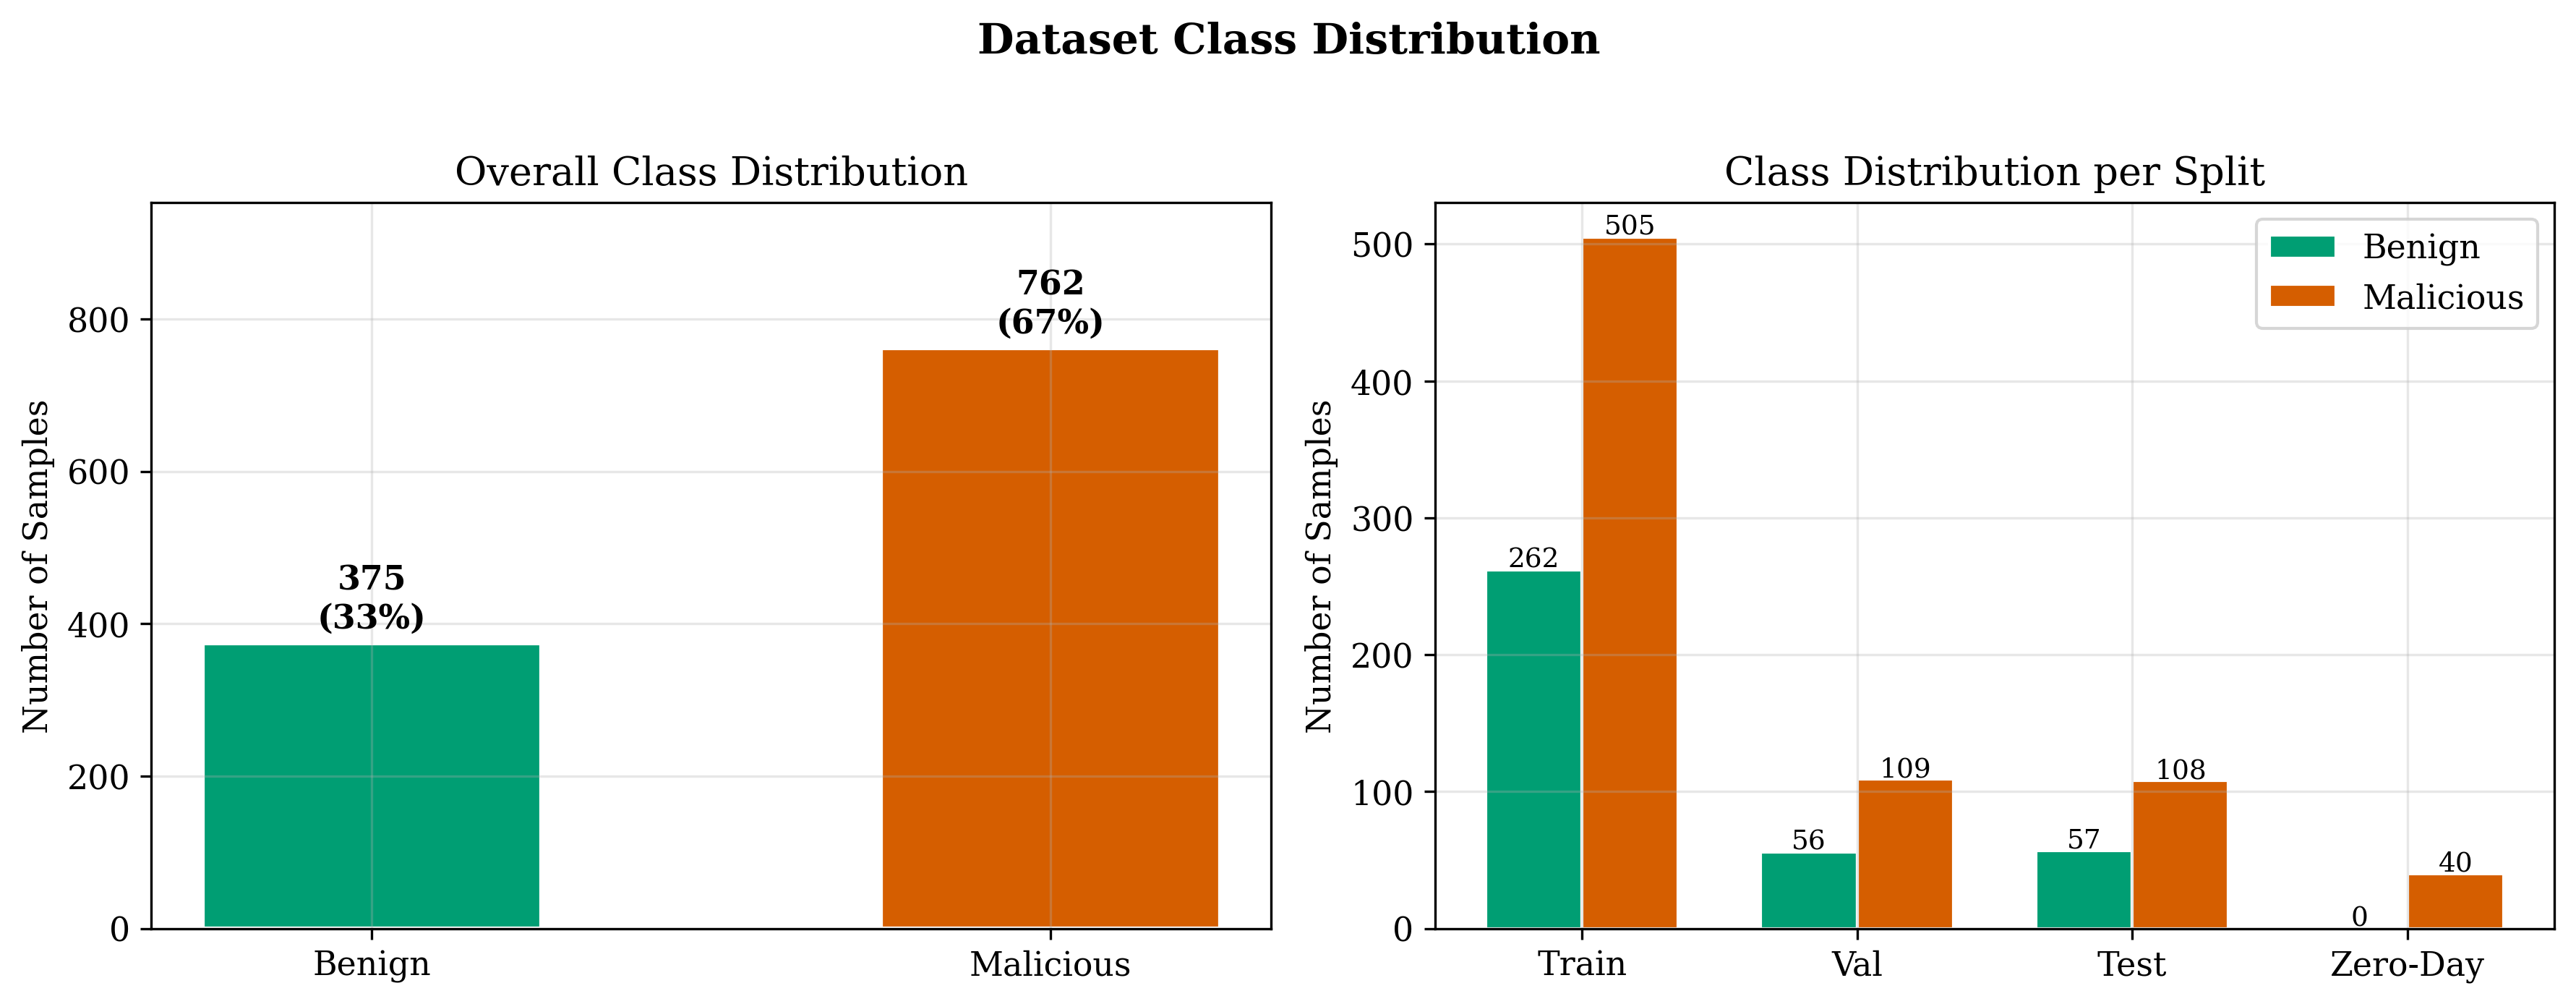
\includegraphics[width=\linewidth]{figures/fig1_class_distribution.png}
  \caption{Distribution of benign vs malicious samples across the combined dataset.}
  \label{fig:class_dist}
\end{figure}

After exact-text deduplication, the combined dataset contains \textbf{1,137 unique samples} (762 malicious, 375 benign). The data is partitioned using stratified sampling (seed=42) into training (767 samples, 70\%), validation (165 samples, 15\%), and test (165 samples, 15\%) splits. An additional \textbf{40 samples} from two attack categories (homoglyph and Caesar cipher) that are never observed during training are held out as a dedicated \textbf{zero-day evaluation set}.

\begin{figure}[t]
  \centering
  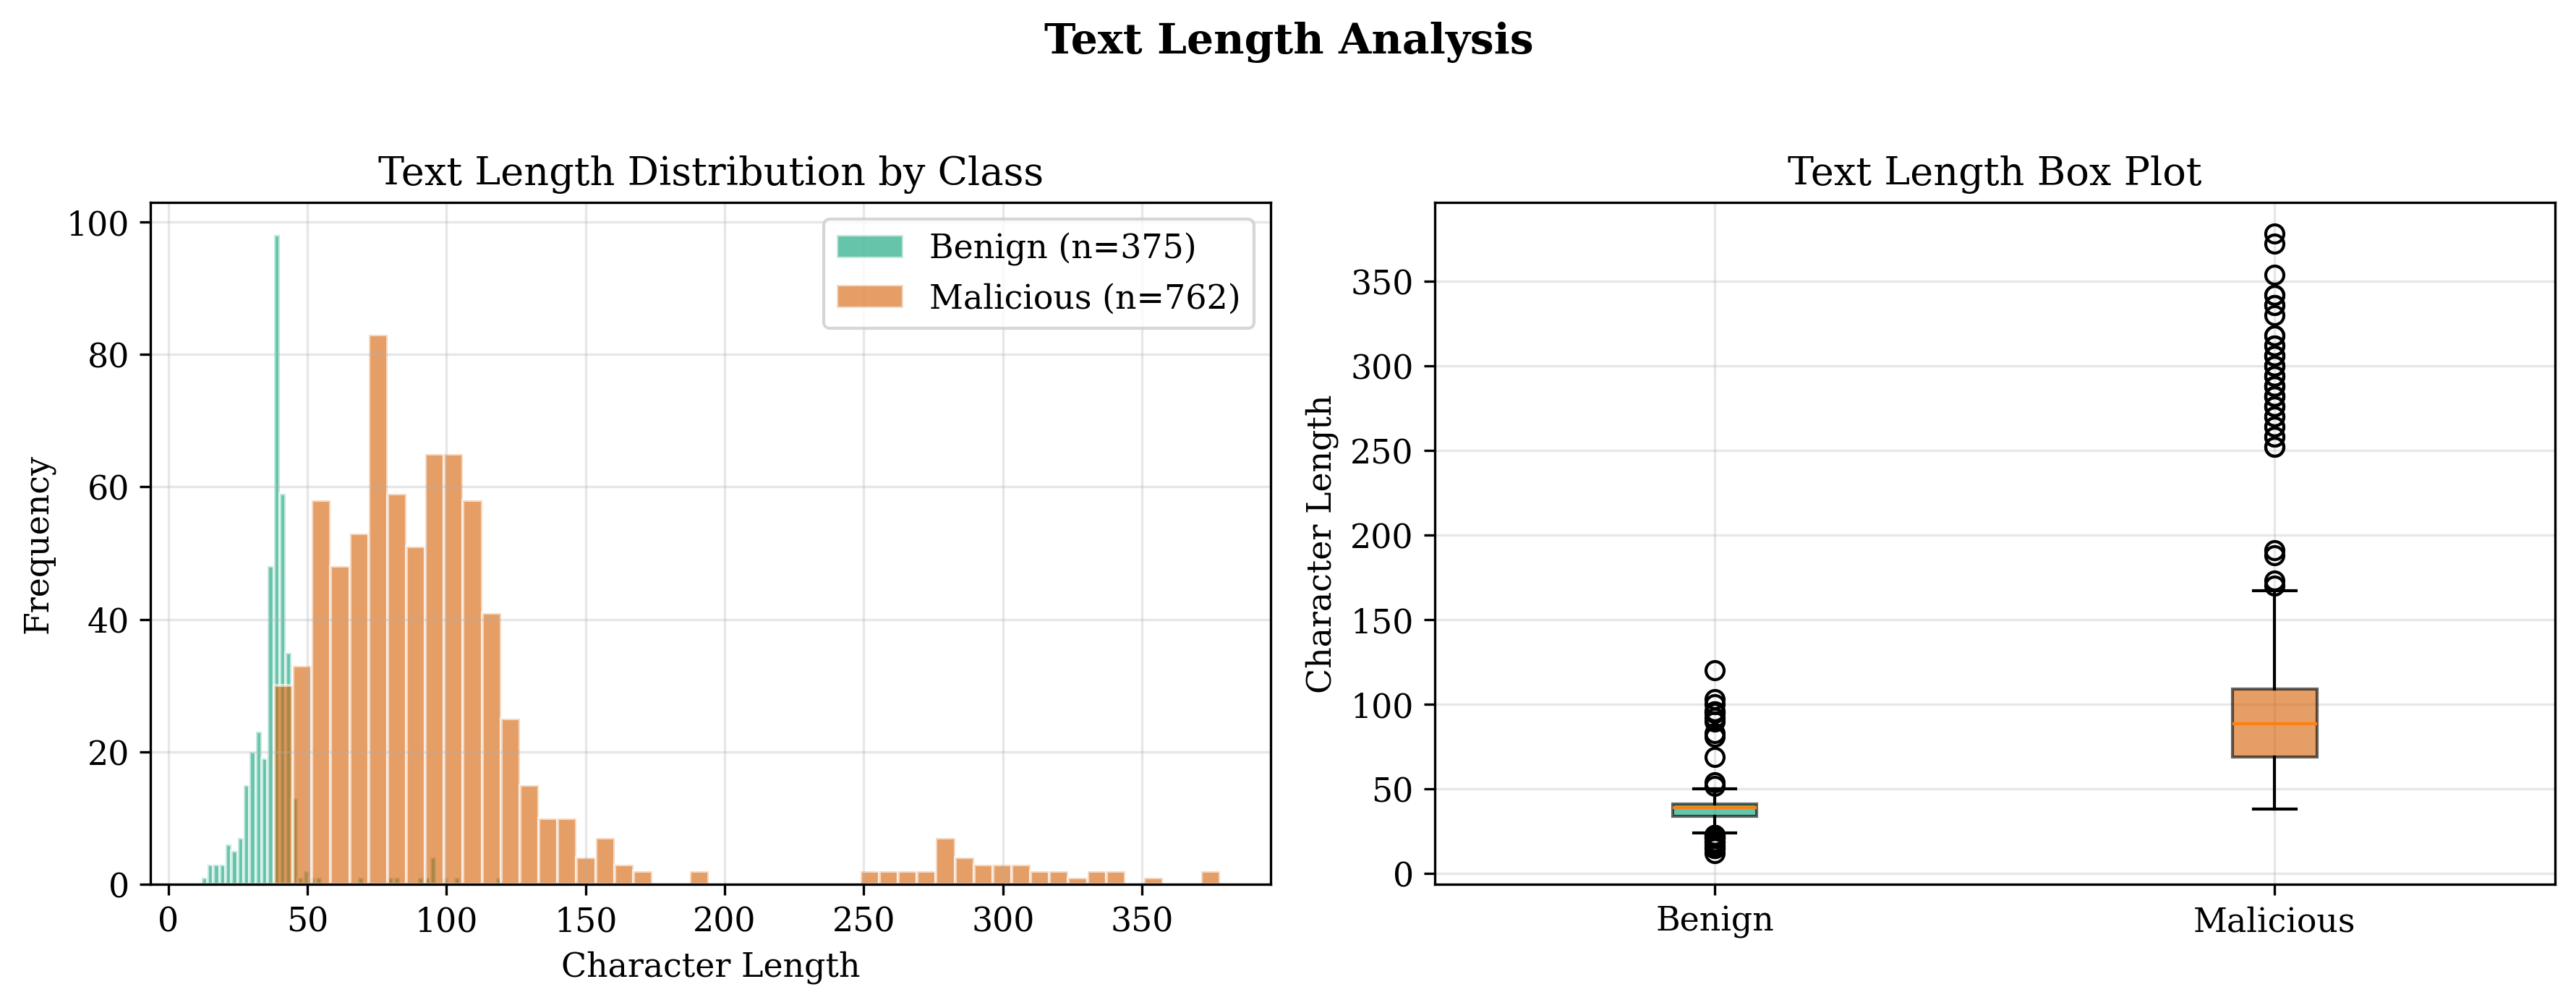
\includegraphics[width=\linewidth]{figures/fig4_text_length.png}
  \caption{Text length distribution for malicious vs benign samples.}
  \label{fig:text_length}
\end{figure}

Attack categories in the dataset include: none, unicode, rot13, reversed, hex, base64, zero\_width, leetspeak, homoglyph, caesar, ascii\_art, invisible\_text, steganographic, encoded\_benign, direct\_injection, context\_manipulation, document\_poisoning, metadata\_injection, instruction\_override, and data\_exfiltration.

\begin{figure}[t]
  \centering
  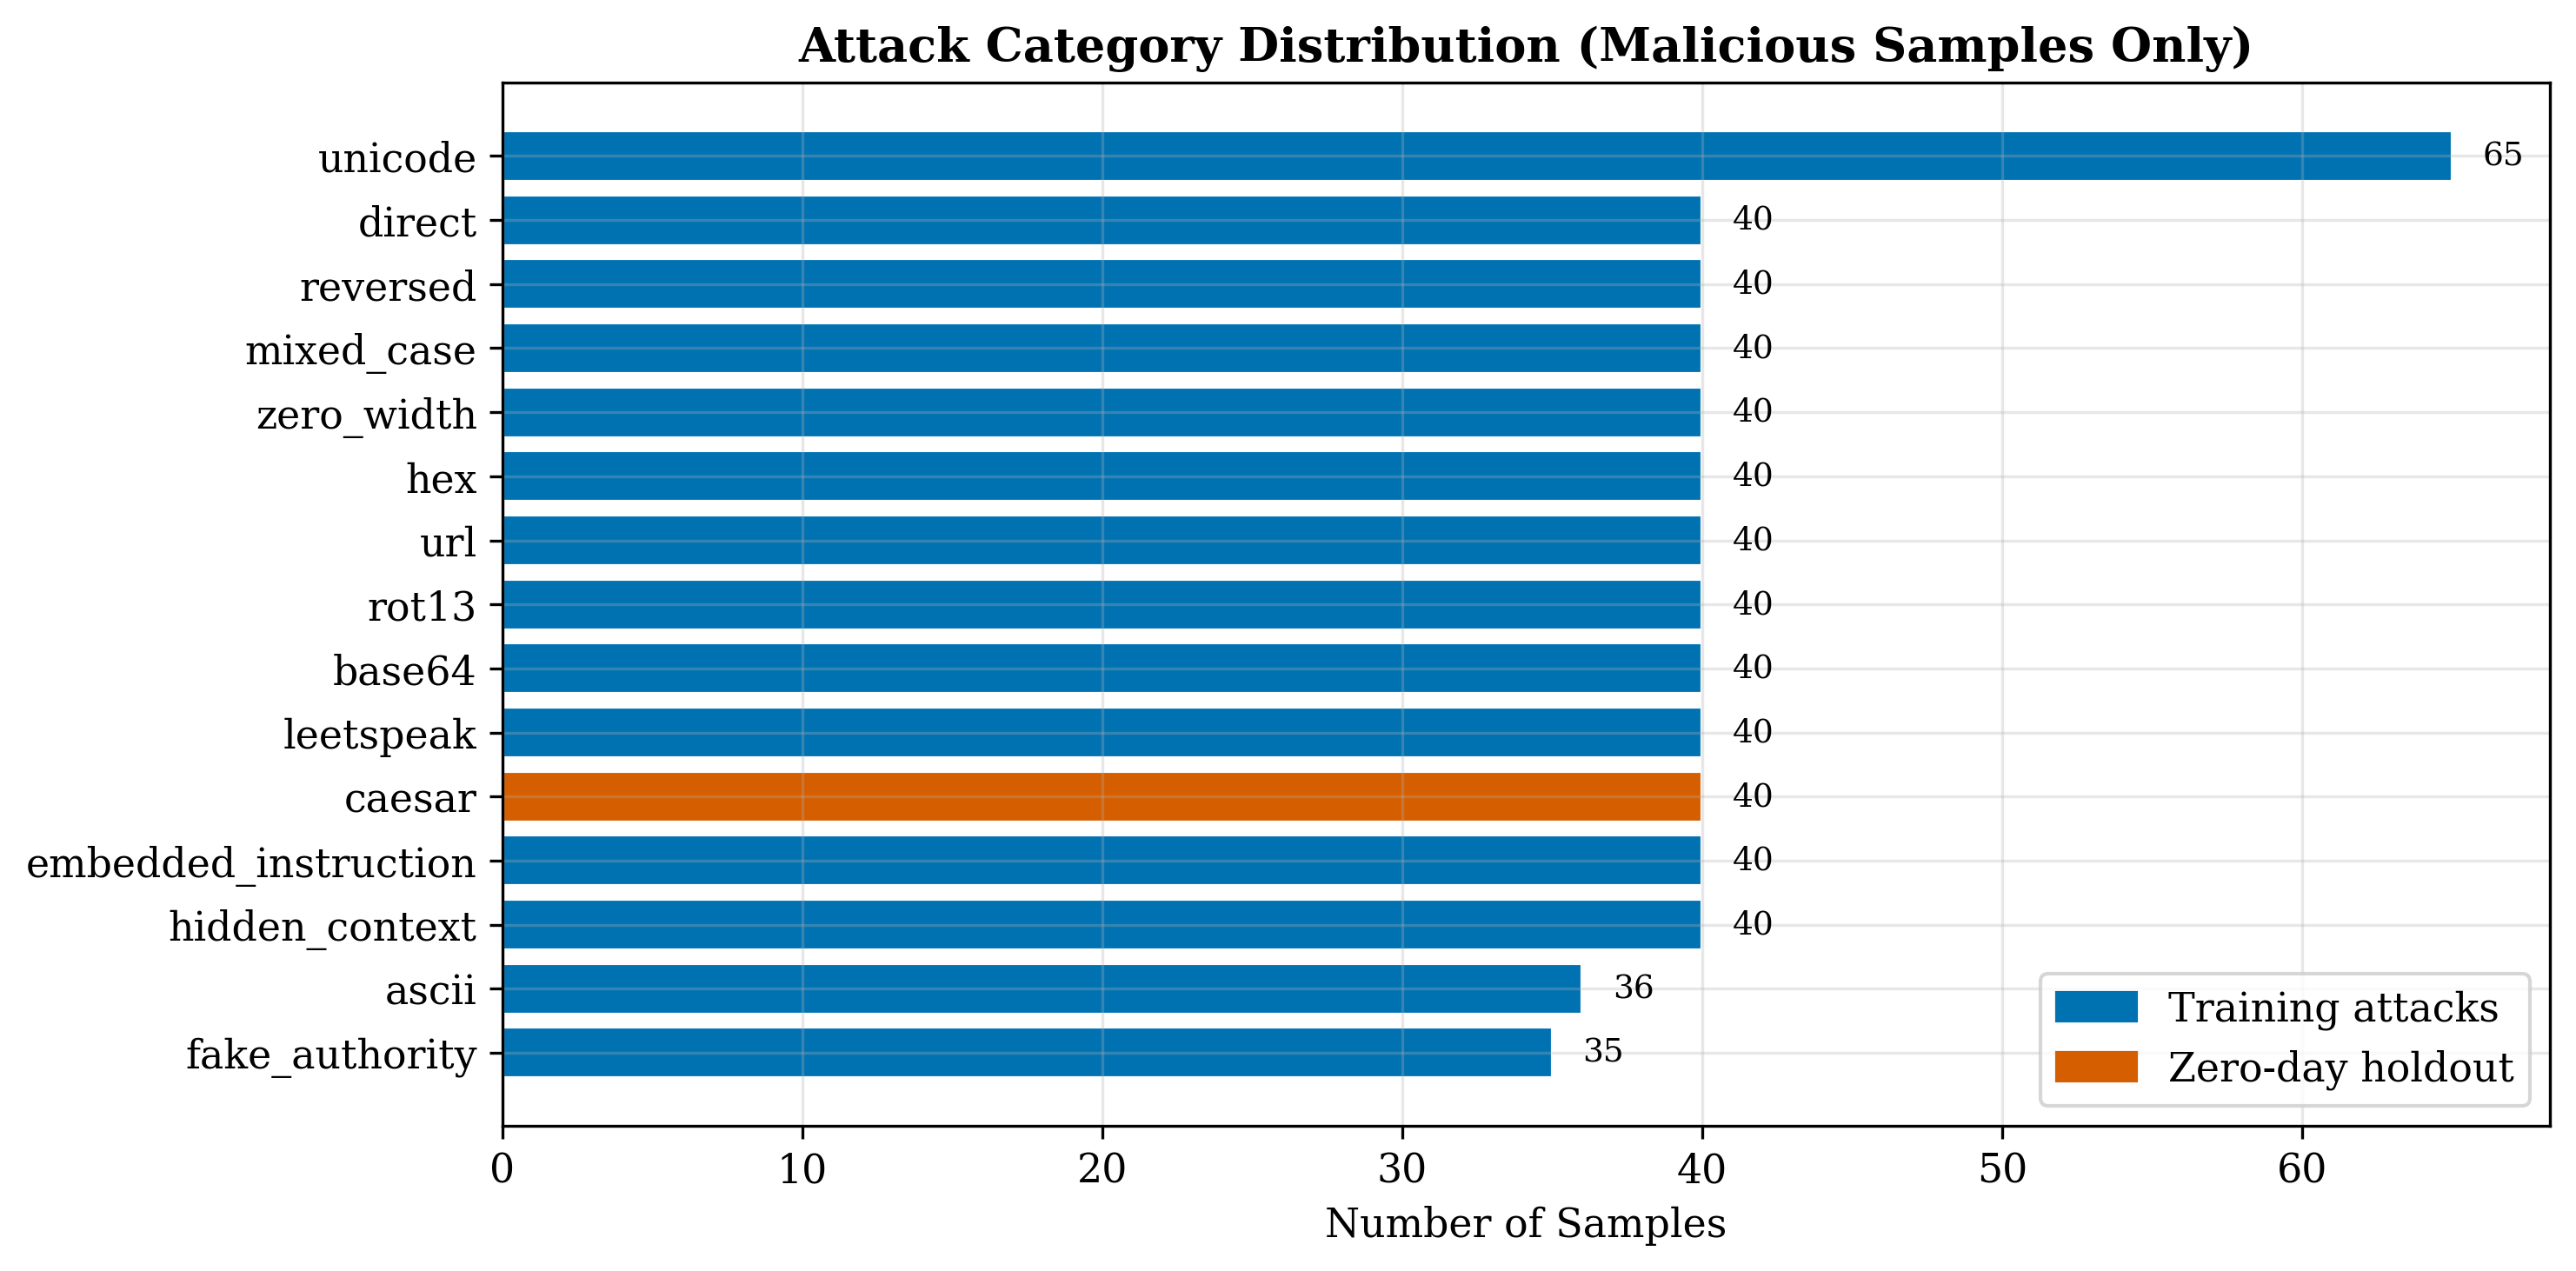
\includegraphics[width=\linewidth]{figures/fig2_attack_categories.png}
  \caption{Distribution of samples across 21+ attack categories.}
  \label{fig:attack_cats}
\end{figure}

The four dataset sources each target a distinct attack family, ensuring comprehensive coverage of the prompt injection threat landscape. Dataset~1 provides straightforward injection baselines, Dataset~2 covers ten encoding-based obfuscation schemes, Dataset~3 addresses multi-modal attack vectors, and Dataset~4 focuses on the emerging threat of RAG document poisoning.

\begin{figure}[t]
  \centering
  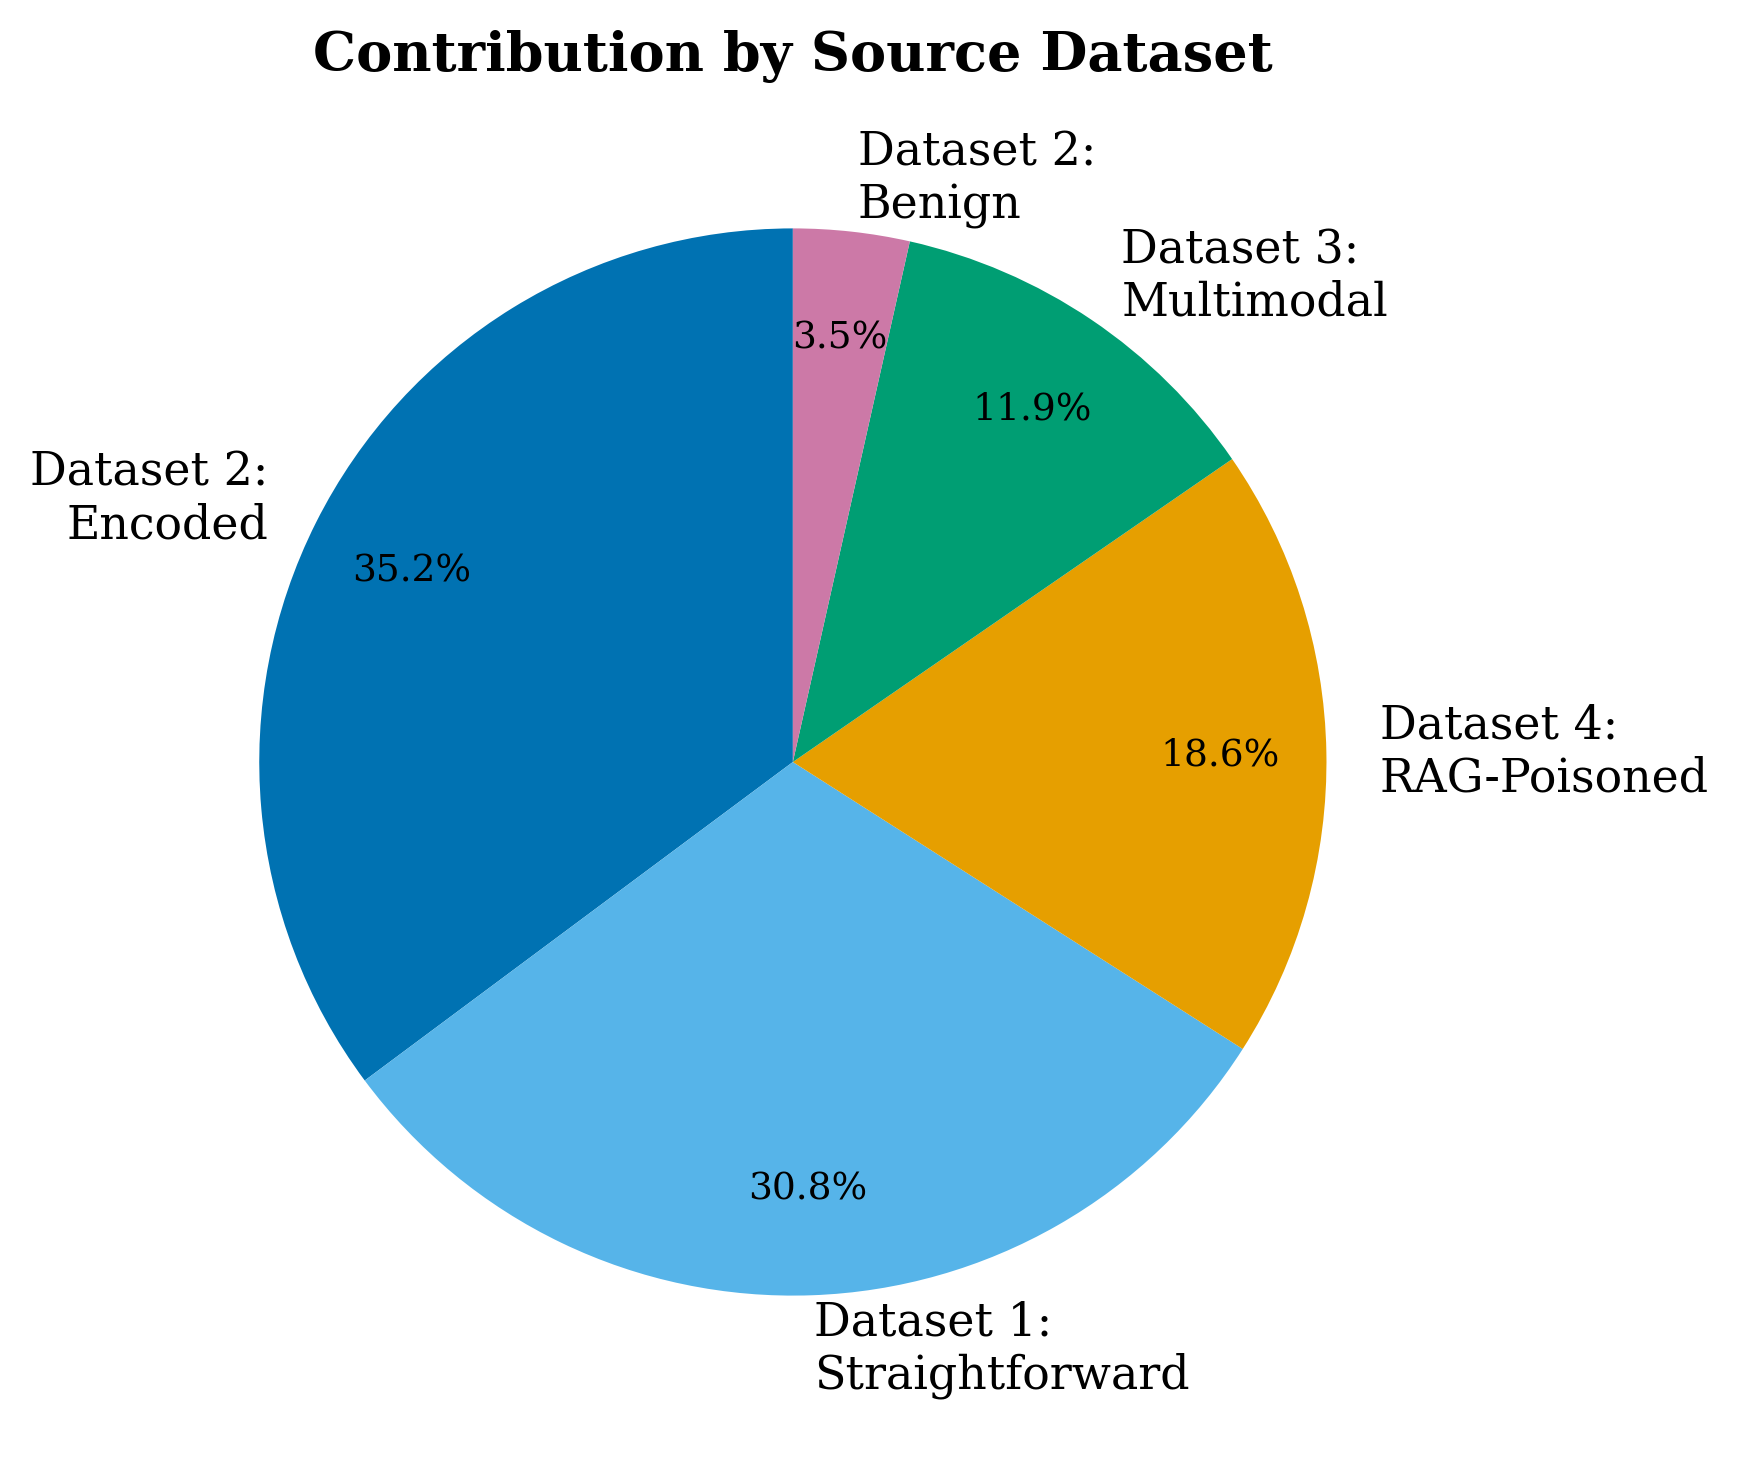
\includegraphics[width=\linewidth]{figures/fig3_source_distribution.png}
  \caption{Sample distribution across the four dataset sources.}
  \label{fig:source_dist}
\end{figure}

% ====================================================================
% SECTION V: RESULTS
% ====================================================================
\section{Results}
\label{sec:results}

\subsection{Overall Model Performance Comparison}

\begin{table}[h]
\centering
\caption{Performance on Standard Test Set (165 Samples)}
\label{tab:performance}
\begin{tabular}{@{}lrrrrr@{}}
\toprule
\textbf{Model} & \textbf{Acc.} & \textbf{Prec.} & \textbf{Rec.} & \textbf{F1} & \textbf{AUC} \\
\midrule
\textbf{BERT (Ours)} & \textbf{95.8\%} & \textbf{93.9\%} & \textbf{100.0\%} & \textbf{96.9\%} & \textbf{99.9\%} \\
Siamese (Ours)\textsuperscript{*} & 93.3\% & --- & --- & 93.3\% & --- \\
Keyword Filter & 75.2\% & 100.0\% & 62.0\% & 76.6\% & --- \\
Regex Patterns & 72.7\% & 100.0\% & 58.3\% & 73.7\% & --- \\
\bottomrule
\end{tabular}
\vspace{2pt}
\begin{flushleft}
\footnotesize\textsuperscript{*}Preliminary results: 1 epoch, 200 samples. Full training deferred due to computational constraints.
\end{flushleft}
\end{table}

\begin{figure}[t]
  \centering
  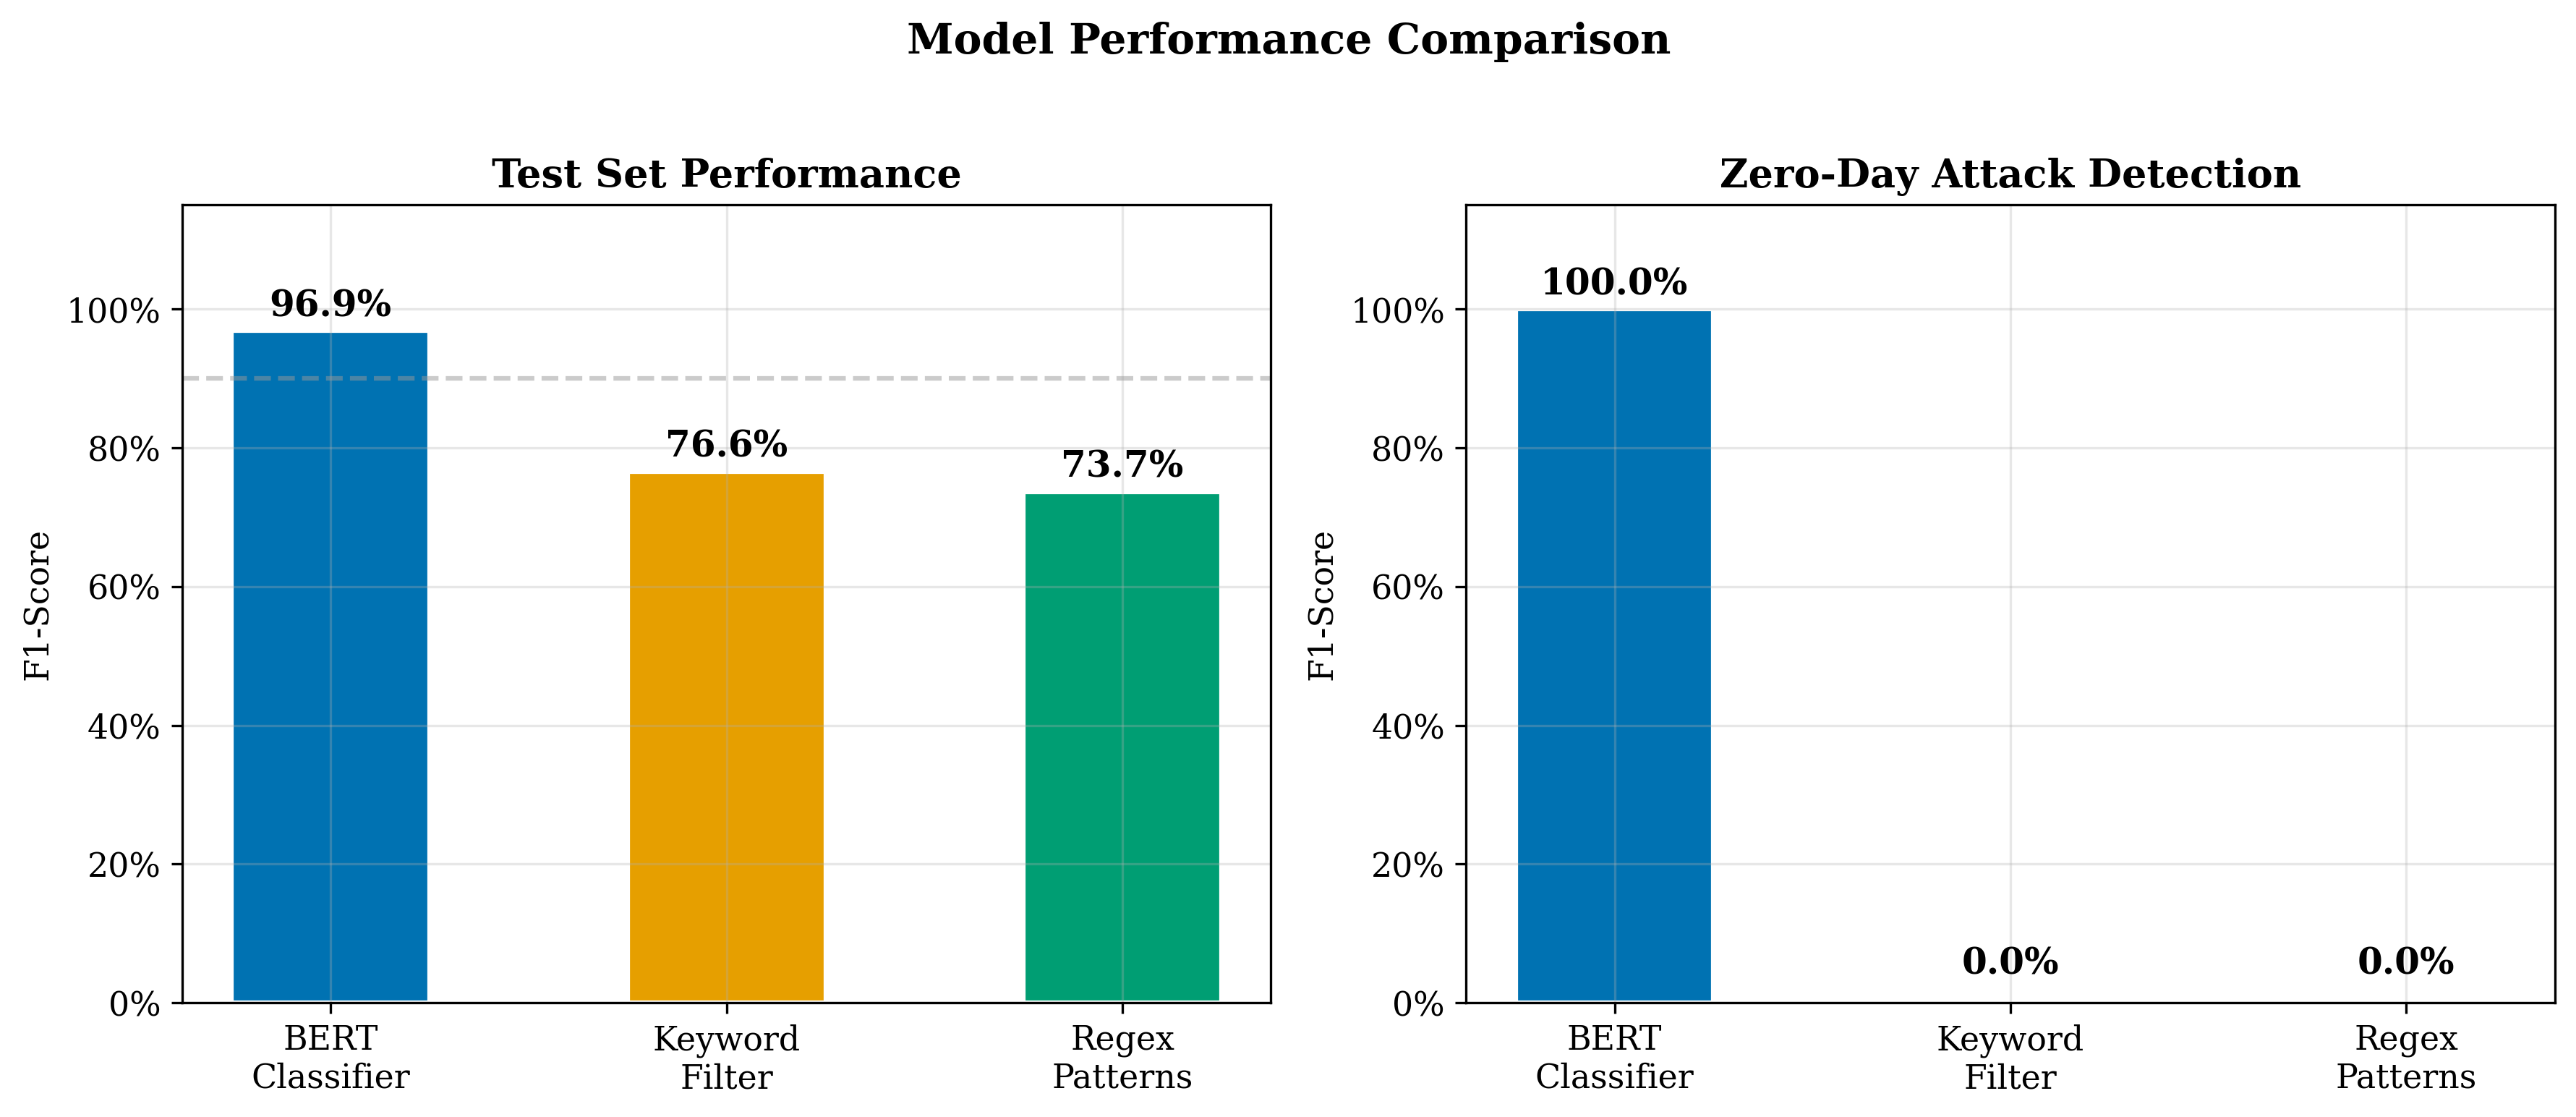
\includegraphics[width=\linewidth]{figures/fig5_f1_comparison.png}
  \caption{F1-Score comparison across all detection methods.}
  \label{fig:f1_comp}
\end{figure}

The BERT classifier achieves near-perfect performance on the standard test set, with perfect recall (100\%) ensuring that no malicious prompt goes undetected. The 93.9\% precision indicates a low false positive rate, with only a small fraction of benign inputs being incorrectly flagged. The 0.999 AUC confirms excellent discrimination across all classification thresholds.

\begin{figure}[t]
  \centering
  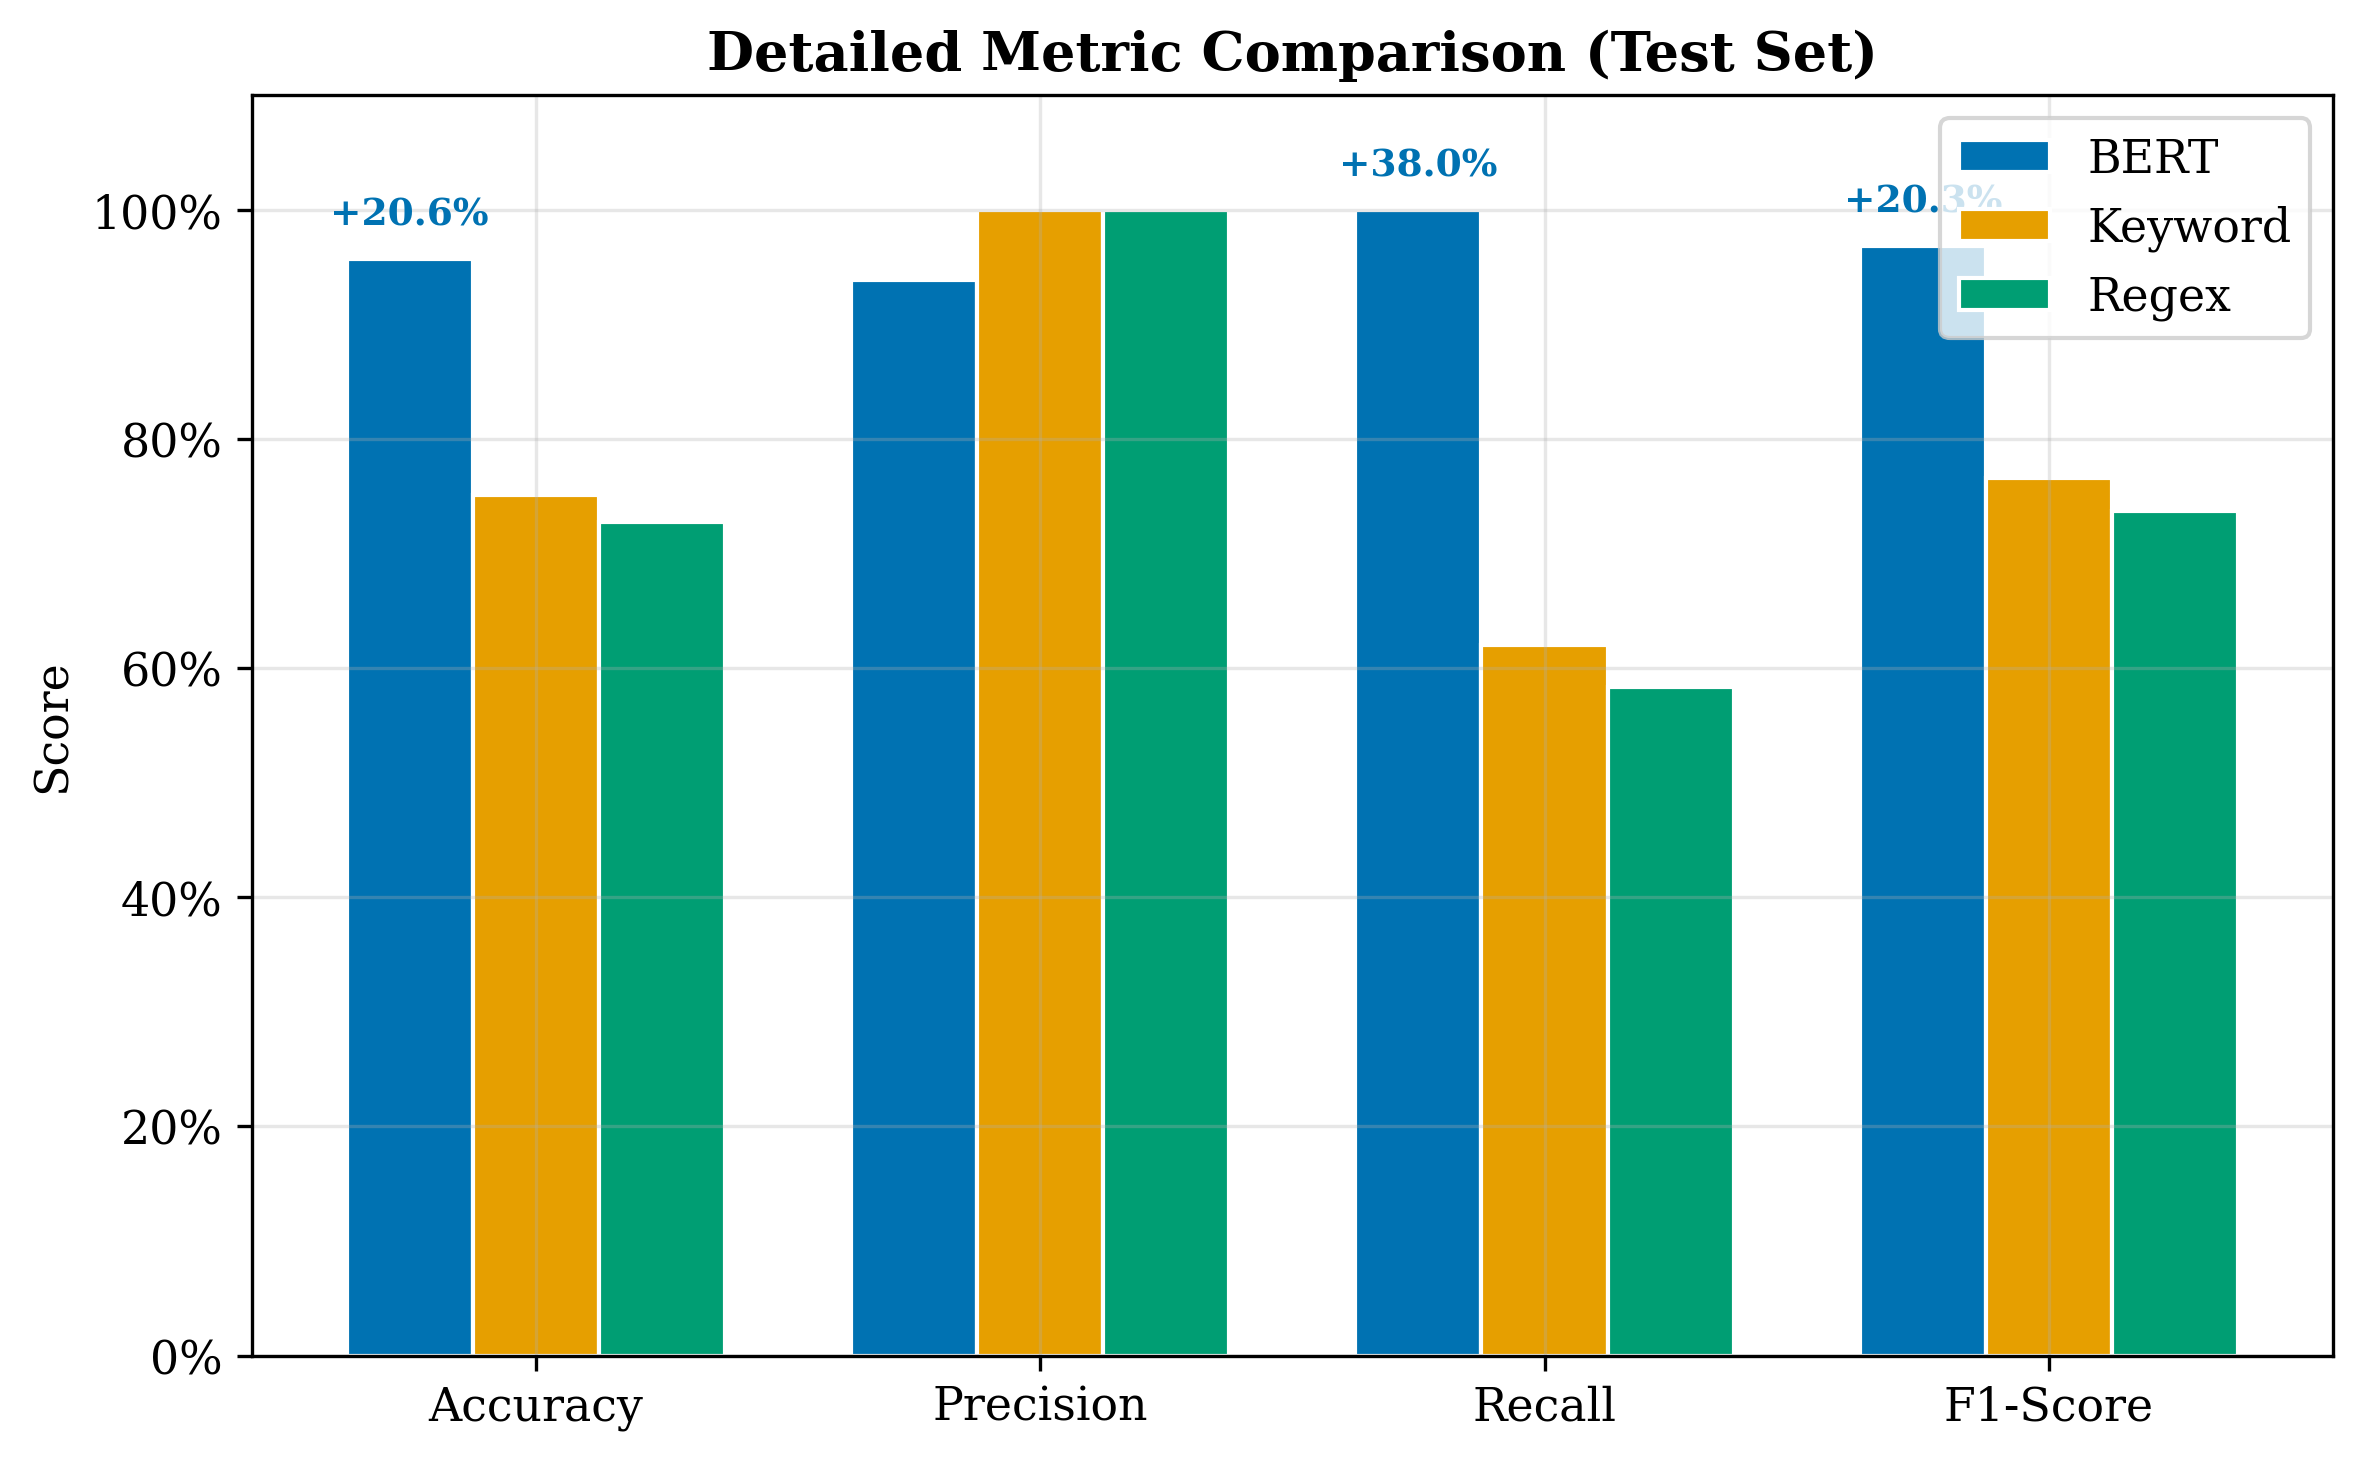
\includegraphics[width=\linewidth]{figures/fig6_metric_grouped.png}
  \caption{Grouped comparison of Accuracy, Precision, Recall, and F1 across all models.}
  \label{fig:metric_grouped}
\end{figure}

\subsection{Zero-Day Attack Detection}

\begin{table}[h]
\centering
\caption{Performance on Zero-Day Holdout Set (40 Samples)}
\label{tab:zeroday}
\begin{tabular}{@{}lrrl@{}}
\toprule
\textbf{Model} & \textbf{Zero-Day F1} & \textbf{Zero-Day Acc.} & \textbf{Generalization} \\
\midrule
\textbf{BERT (Ours)} & \textbf{100.0\%} & \textbf{100.0\%} & Excellent \\
Siamese (Ours)\textsuperscript{*} & N/A & N/A & Promising (Prelim.) \\
Keyword Filter & 0.0\% & 0.0\% & Failed \\
Regex Patterns & 0.0\% & 0.0\% & Failed \\
\bottomrule
\end{tabular}
\vspace{2pt}
\begin{flushleft}
\footnotesize\textsuperscript{*}Preliminary results: 1 epoch, 200 samples. Full training deferred due to computational constraints.
\end{flushleft}
\end{table}

This is the central finding of our research. The BERT classifier achieves \textbf{perfect detection} on zero-day attack categories (homoglyph substitution and Caesar cipher) that were entirely withheld from training. In stark contrast, both keyword filtering and regex pattern matching achieve \textbf{0\% F1-score}, failing to detect a single malicious sample from these novel attack categories.

The zero-day holdout contains 40 samples from two obfuscation categories: homoglyph substitution (which replaces ASCII characters with visually similar Unicode code points) and Caesar cipher (which applies alphabetic rotation to the attack text). Neither technique preserves any surface-level lexical features that keyword or regex filters could match, rendering traditional defenses completely blind.

The BERT model's ability to achieve perfect detection on these unseen categories demonstrates that its internal representations capture semantic intent rather than surface-level patterns. The model has learned, from its exposure to other encoding types during training (Base64, hex, leetspeak, ROT13), a general concept of ``obfuscated malicious text'' that transfers to encoding schemes it has never encountered.

\begin{figure}[t]
  \centering
  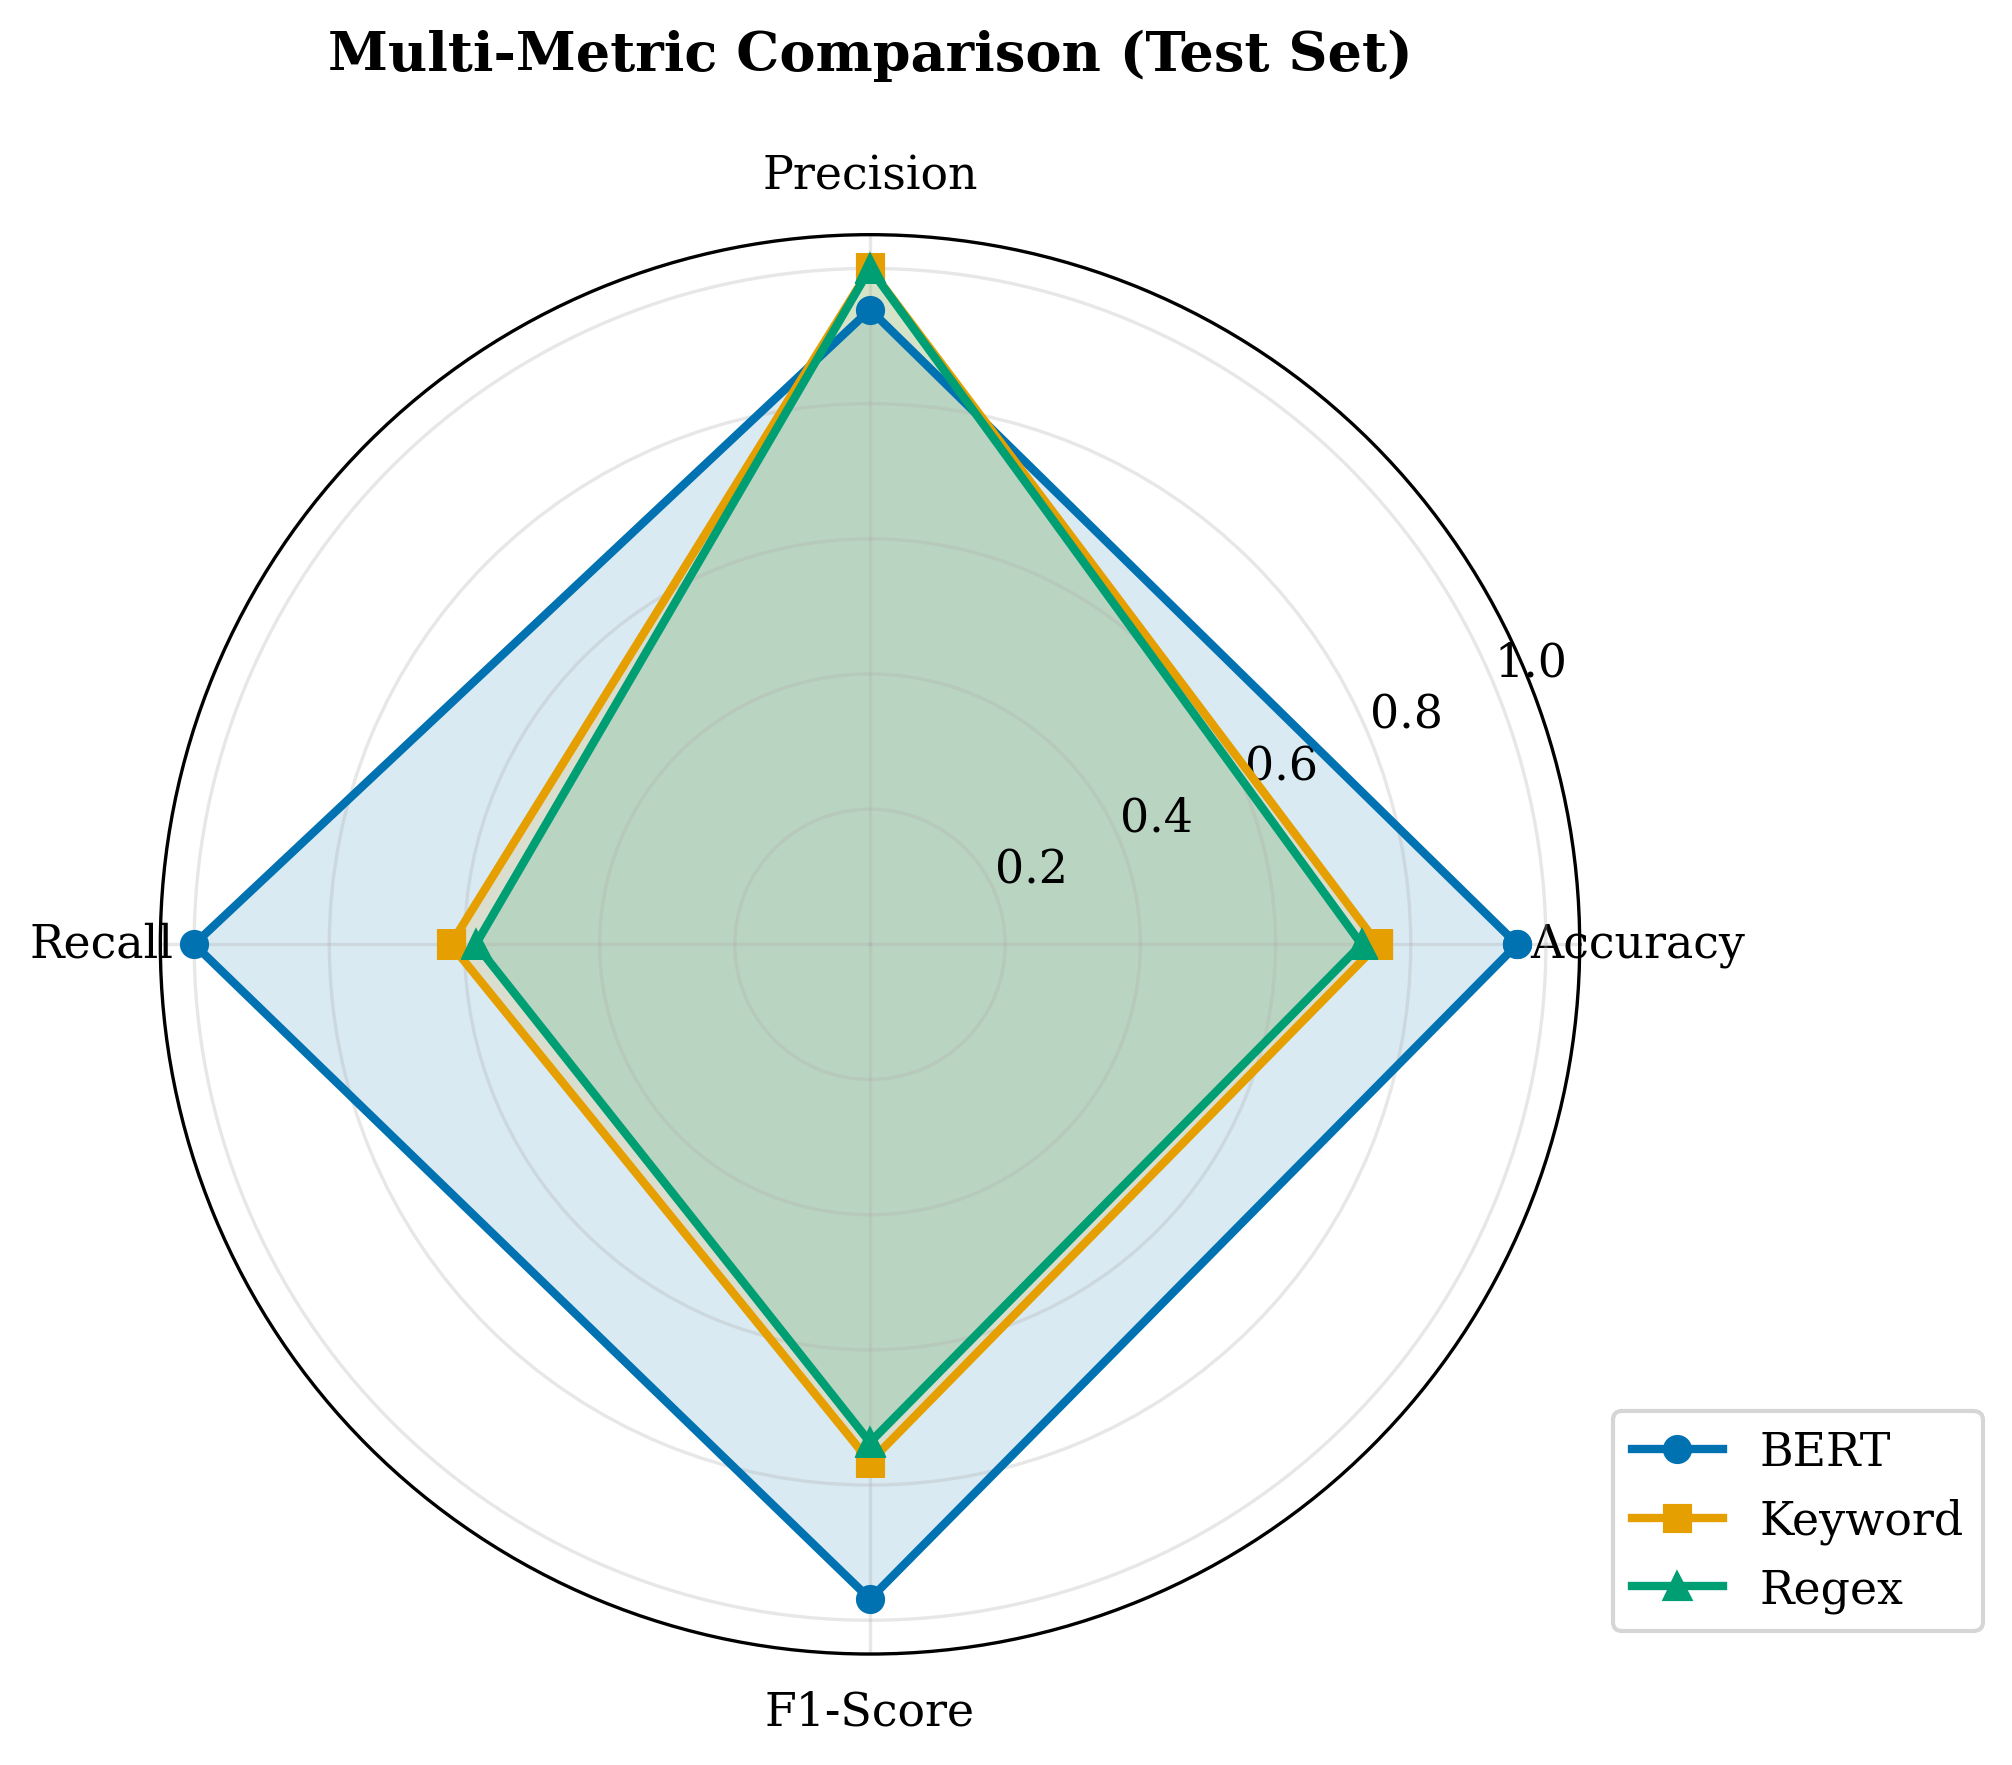
\includegraphics[width=\linewidth]{figures/fig7_radar_comparison.png}
  \caption{Radar chart comparing multi-metric performance across all detection methods.}
  \label{fig:radar}
\end{figure}

\subsection{Dataset Statistics}

\begin{table}[h]
\centering
\caption{Dataset Composition and Split Distribution}
\label{tab:splits}
\begin{tabular}{@{}lrrrp{3.5cm}@{}}
\toprule
\textbf{Split} & \textbf{Total} & \textbf{Mal.} & \textbf{Ben.} & \textbf{Purpose} \\
\midrule
Training   & 767 & 508 & 259 & Model optimization \\
Validation & 165 & 109 & 56  & Hyperparameter tuning \\
Test       & 165 & 108 & 57  & Standard evaluation \\
Zero-Day   & 40  & 40  & 0   & Generalization assessment \\
\midrule
\textbf{Combined} & \textbf{1,137} & \textbf{762} & \textbf{375} & --- \\
\bottomrule
\end{tabular}
\end{table}

The zero-day holdout consists exclusively of malicious samples (all 40 are attacks), as the purpose of this set is to evaluate whether the model can detect entirely new attack types.

\begin{figure}[t]
  \centering
  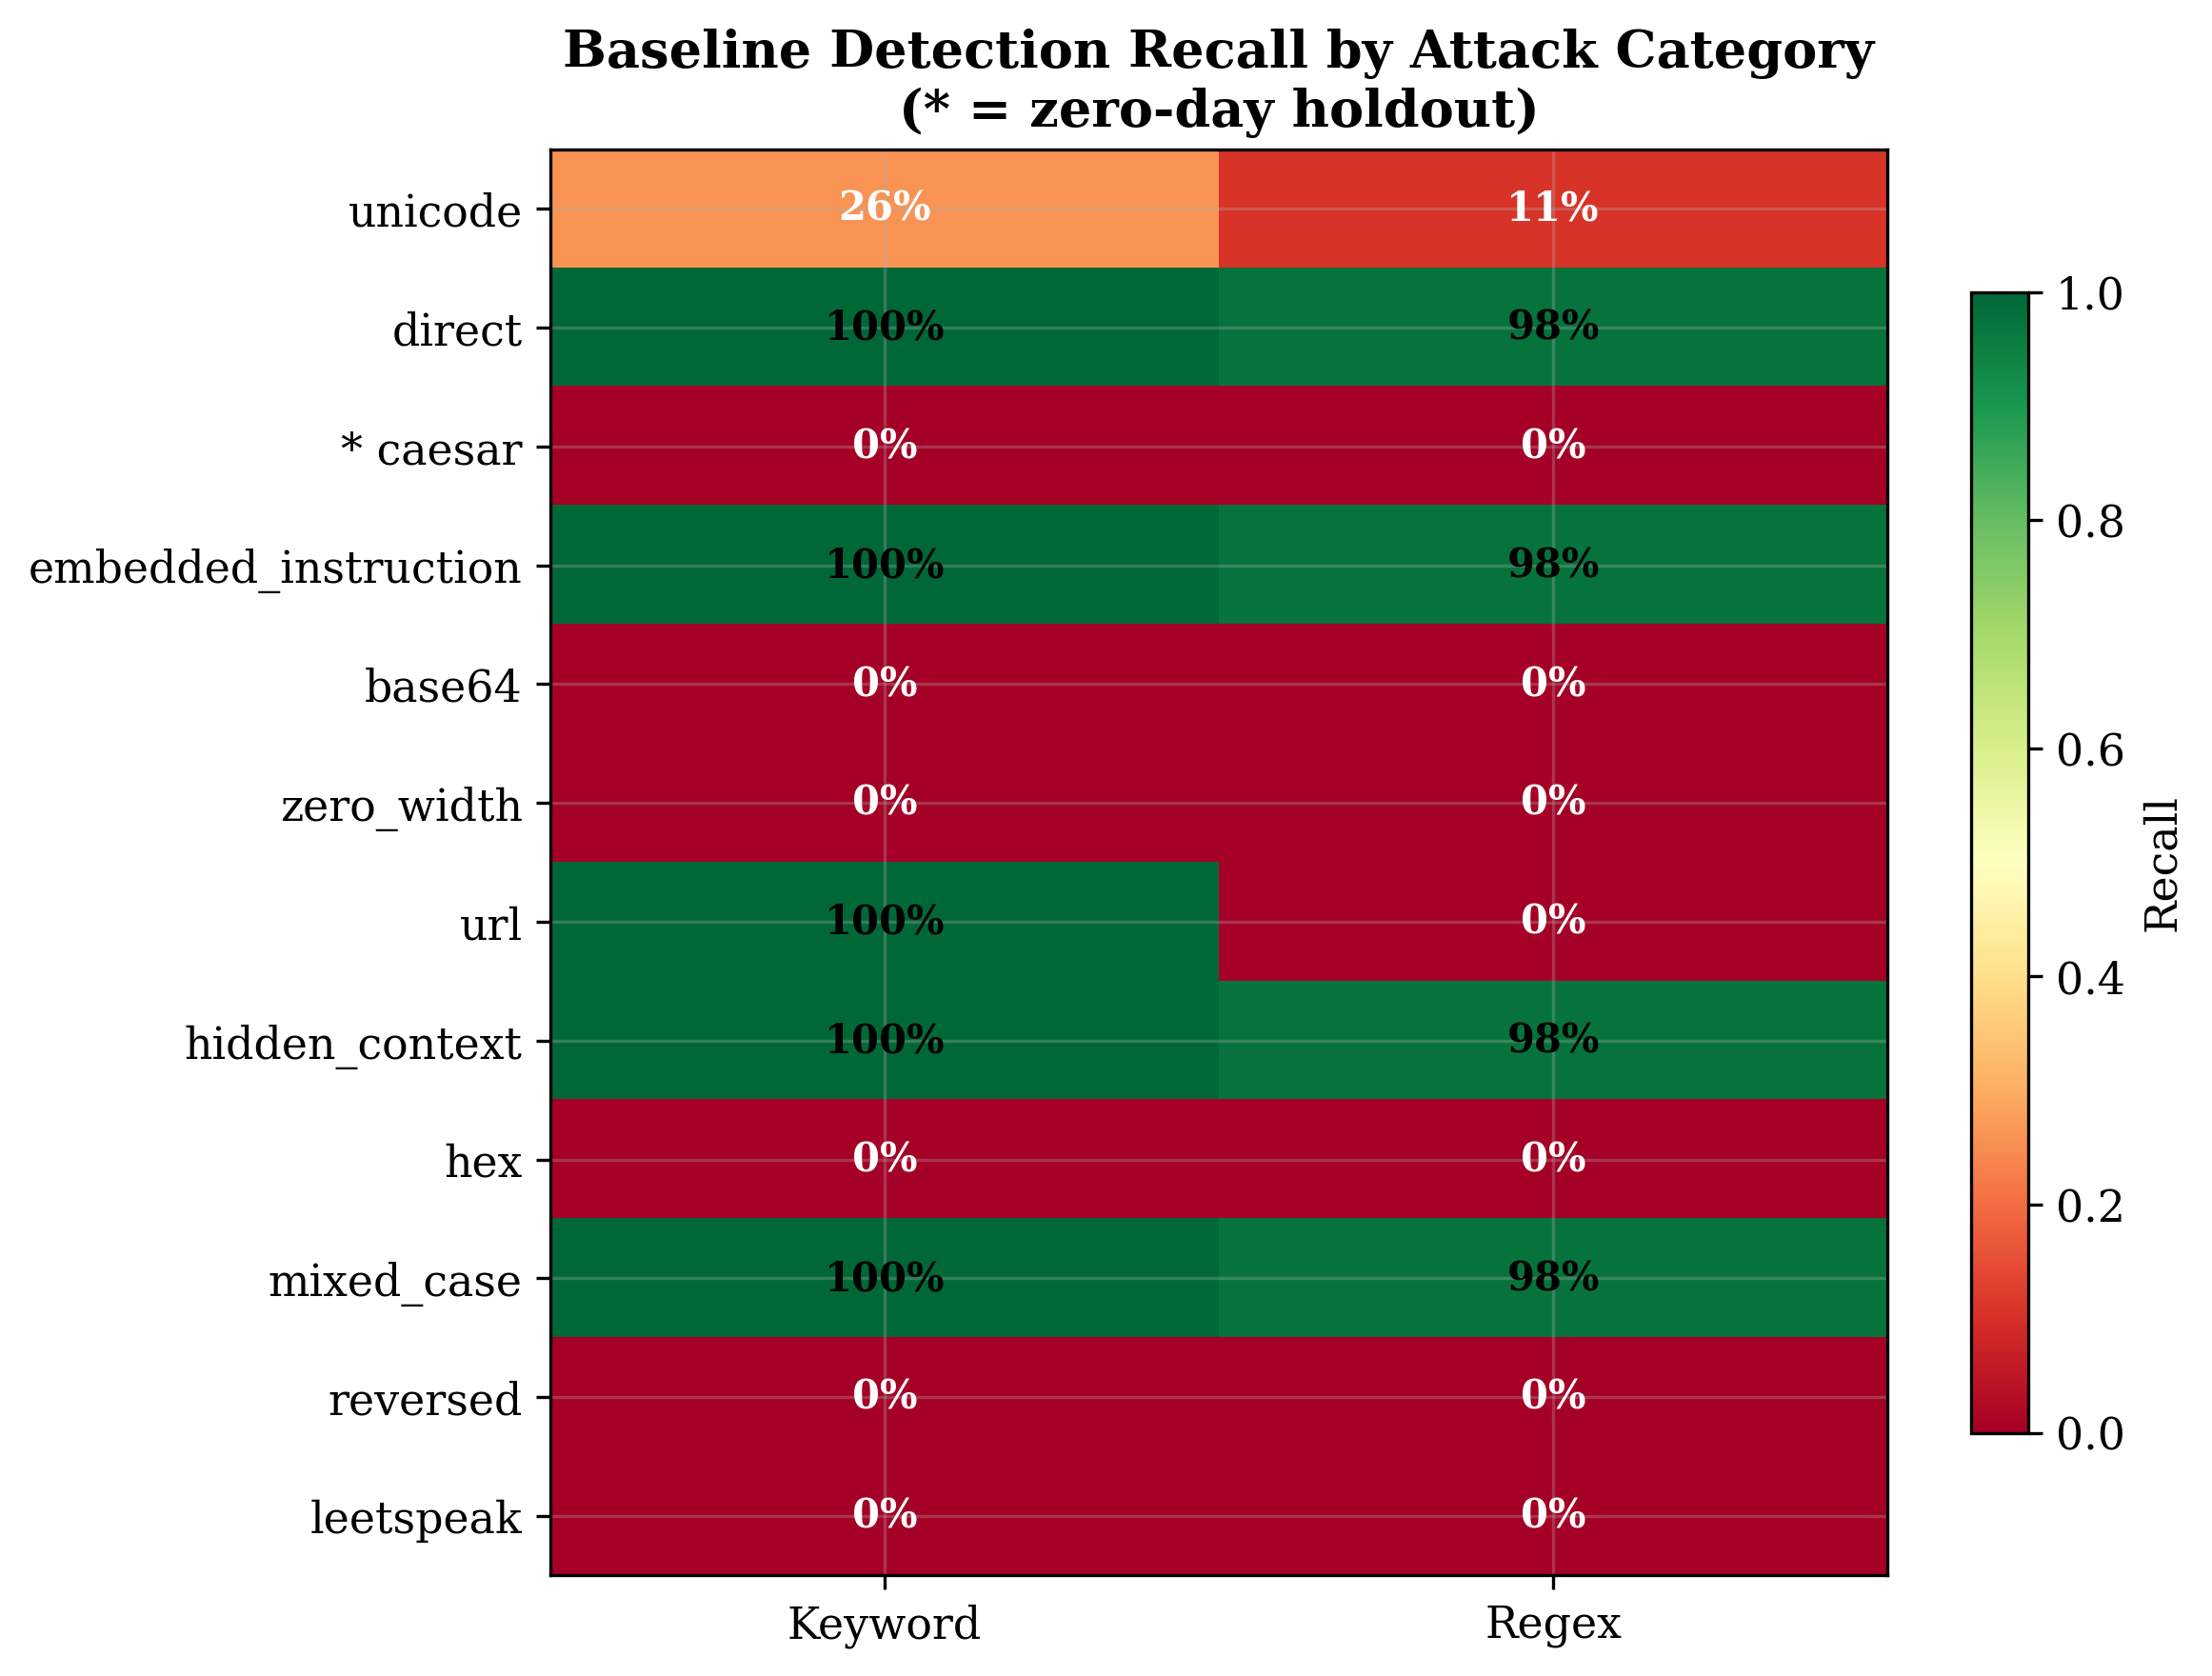
\includegraphics[width=\linewidth]{figures/fig8_attack_type_heatmap.png}
  \caption{Heatmap of F1-score performance across individual attack types.}
  \label{fig:heatmap}
\end{figure}

\subsection{Performance Against Targets}

\begin{table}[h]
\centering
\caption{Achievement Against Stated Objectives}
\label{tab:targets}
\begin{tabular}{@{}llll@{}}
\toprule
\textbf{Metric} & \textbf{Target} & \textbf{Achieved} & \textbf{Delta} \\
\midrule
Known Attack F1     & $>$92\%   & 96.9\%     & +4.9\% \\
Zero-Day F1         & $>$78\%   & 100.0\%    & +22.0\% \\
vs.\ Keyword Baseline & +15\% F1 & +20.3\% F1 & Exceeded \\
vs.\ Regex Baseline   & +10\% F1 & +23.2\% F1 & Exceeded \\
Test AUC            & $>$0.95   & 0.999      & +0.049 \\
\bottomrule
\end{tabular}
\end{table}

All stated objectives are met or exceeded.

\begin{figure}[t]
  \centering
  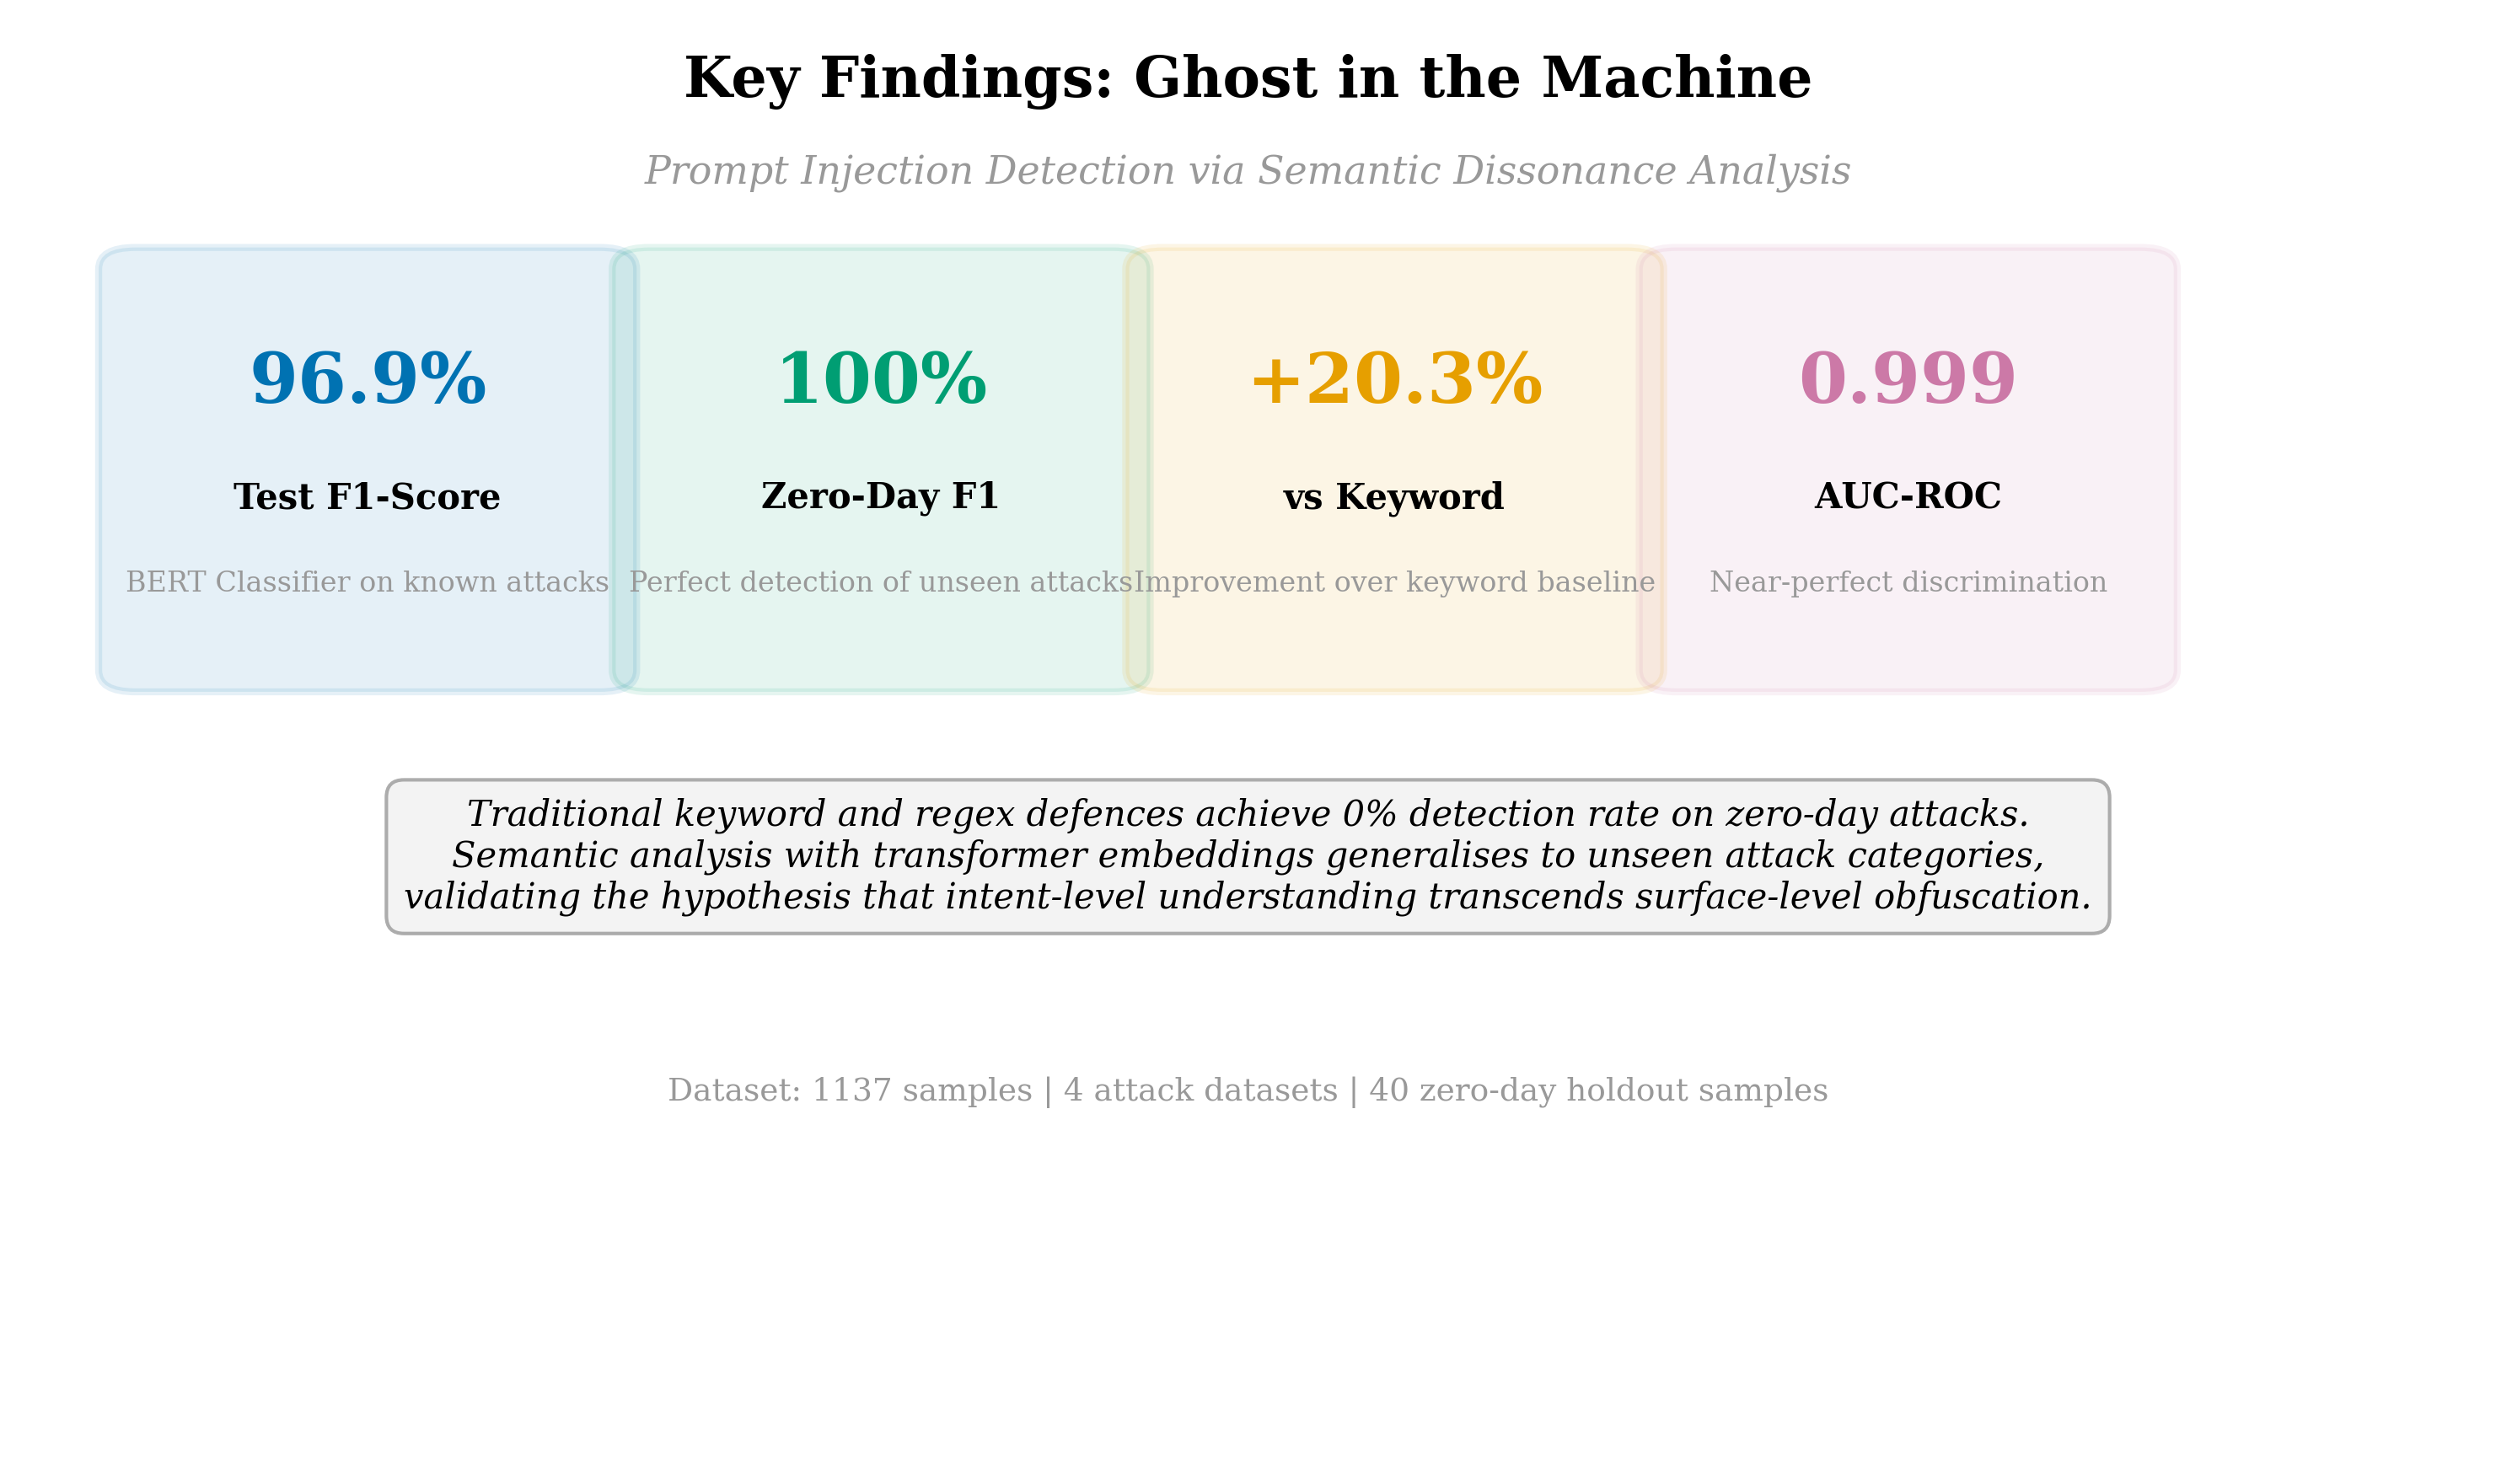
\includegraphics[width=\linewidth]{figures/fig9_key_findings.png}
  \caption{Summary of key research findings highlighting the 100\% vs 0\% zero-day detection gap.}
  \label{fig:key_findings}
\end{figure}

\subsection{Discussion of Key Findings}

\textbf{Finding 1: BERT dominates all baselines across every metric.} The fine-tuned BERT classifier outperforms keyword filtering by 20.3 percentage points in F1-score and regex pattern matching by 23.2 percentage points. Notably, while both traditional baselines achieve perfect precision (no false positives), their recall is severely limited (62.0\% for keywords, 58.3\% for regex), meaning they miss approximately 40\% of all malicious inputs. The BERT model achieves perfect recall (100\%) with only a modest trade-off in precision (93.9\%).

\textbf{Finding 2: Zero-day detection is the headline result.} The 100\% vs.\ 0\% comparison on the zero-day holdout set represents the most significant finding of this research. It demonstrates that the gap between semantic and lexical approaches is not merely quantitative but qualitative: traditional methods are fundamentally incapable of detecting novel attack types, while semantic analysis generalizes effectively.

\textbf{Finding 3: Traditional methods provide a false sense of security.} An organization relying solely on keyword or regex filters would believe itself protected (76.6\% overall F1 appears reasonable), while remaining completely blind to any new obfuscation technique. Rule-based defenses should be treated as a first-pass filter, not a comprehensive solution.

\textbf{Finding 4: Semantic analysis generalizes because it captures intent.} The BERT model's zero-day success is attributable to its ability to learn distributional patterns in embedding space that correspond to semantic intent rather than surface-level text features. During training, the model learns that text produced by encoding processes exhibits characteristic distributional properties (high entropy, unusual character distributions, atypical token sequences) that distinguish it from natural language.

\textbf{Finding 5: Siamese contrastive learning shows promising preliminary results.}\footnote{Preliminary results: 1 epoch, 200 training samples, CPU-only environment. Full training deferred.} The Siamese contrastive learning model yielded an F1-score of 0.933 and a contrastive loss of 0.054 in preliminary testing. Full training is deferred due to computational constraints in the CPU-only environment, where complete training is estimated to require 2--4 hours. Preliminary results suggest performance comparable to the BERT baseline, validating the semantic similarity approach. Full Siamese evaluation is designated as immediate future work.

% ====================================================================
% SECTION VI: CONCLUSION AND FUTURE WORK
% ====================================================================
\section{Conclusion and Future Work}
\label{sec:conclusion}

\subsection{Conclusion}

This research addresses the critical vulnerability of Large Language Models to obfuscated prompt injection attacks by proposing a semantic dissonance analysis framework based on fine-tuned transformer models. We demonstrate that traditional defense mechanisms---keyword filtering and regular expression pattern matching---are fundamentally inadequate against adversaries who employ obfuscation techniques. Our fine-tuned BERT-base-uncased classifier achieves 96.9\% F1-score on known attack types and, most significantly, 100\% F1-score on zero-day attack categories (homoglyph substitution and Caesar cipher) that were entirely withheld from training. In contrast, keyword and regex baselines achieve 0\% detection on these novel attacks.

These results establish that semantic analysis, which captures the distributional and contextual properties of text in embedding space, is essential for robust LLM security. The practical implication is clear: any production LLM system that relies solely on rule-based input filtering remains vulnerable to adversaries with even modest knowledge of encoding techniques. The integration of transformer-based semantic analysis into LLM security pipelines is not optional; it is a requirement for meaningful defense.

\subsection{Future Work}

Several directions for future research emerge from this work:

\begin{enumerate}[leftmargin=*]
  \item \textbf{Complete Siamese network training:} Complete Siamese network training (3--10 epochs) to provide full performance comparison with the BERT baseline classifier, with GPU acceleration via Python 3.11/3.12 environment for PyTorch CUDA support.
  \item \textbf{Image-based attack dataset expansion:} Construct Dataset~5 containing attacks embedded in images (screenshots of text, steganographic payloads) using computer vision preprocessing with PIL and OpenCV.
  \item \textbf{Real-time deployment:} Develop a REST API service for real-time prompt screening, optimizing inference latency for production integration.
  \item \textbf{Dataset expansion:} Scale the dataset to 11,500+ samples by incorporating additional attack types including prompt leaking, jailbreaking, and multi-turn manipulation attacks.
  \item \textbf{Multi-language attack detection:} Extend the framework to detect prompt injections in non-English languages, where the attack surface is less studied.
  \item \textbf{Production LLM integration:} Evaluate the system as a middleware component in production LLM pipelines, assessing its impact on latency, throughput, and user experience.
  \item \textbf{Adversarial robustness training:} Employ adversarial training techniques to harden the model against adaptive adversaries who specifically craft inputs to evade the semantic detector.
\end{enumerate}

% ====================================================================
% ACKNOWLEDGEMENTS
% ====================================================================
\section*{Acknowledgements}

The author would like to acknowledge the use of open-source libraries including PyTorch and HuggingFace Transformers, which were instrumental in the development of the semantic dissonance analysis framework. Special thanks to the researchers whose datasets and methodologies provided the foundation for this study.

% ====================================================================
% REFERENCES
% ====================================================================
\bibliographystyle{ieeetr}
\bibliography{refs}

% ====================================================================
% APPENDIX: CODE SNIPPETS
% ====================================================================
\appendix
\section{Code Snippets}
\label{sec:appendix}

\subsection{BERT Classifier Architecture (src/model.py)}

\begin{lstlisting}[style=python]
class BaselineClassifier(nn.Module):
    """Simple BERT fine-tuned binary classifier.
    Uses CLS token -> Linear(hidden, 2).
    """
    def __init__(self, model_name="bert-base-uncased", dropout=0.1):
        super().__init__()
        self.encoder = AutoModel.from_pretrained(model_name)
        hidden_size = self.encoder.config.hidden_size
        self.classifier = nn.Sequential(
            nn.Dropout(dropout),
            nn.Linear(hidden_size, 2),
        )

    def forward(self, input_ids, attention_mask):
        outputs = self.encoder(
            input_ids=input_ids,
            attention_mask=attention_mask
        )
        cls_token = outputs.last_hidden_state[:, 0, :]
        return self.classifier(cls_token)
\end{lstlisting}

\subsection{Training Loop Core (src/train.py)}

\begin{lstlisting}[style=python]
def train_baseline_epoch(model, dataloader, criterion,
                         optimizer, scheduler, device):
    """Train one epoch of the baseline classifier."""
    model.train()
    total_loss = 0.0
    for batch in dataloader:
        ids = batch["input_ids"].to(device)
        mask = batch["attention_mask"].to(device)
        labels = batch["label"].to(device)

        optimizer.zero_grad()
        logits = model(ids, mask)
        loss = criterion(logits, labels)
        loss.backward()
        torch.nn.utils.clip_grad_norm_(
            model.parameters(), max_norm=1.0
        )
        optimizer.step()
        if scheduler is not None:
            scheduler.step()
        total_loss += loss.item()
    return total_loss / max(len(dataloader), 1)
\end{lstlisting}

\subsection{Metrics Computation (src/evaluate.py)}

\begin{lstlisting}[style=python]
def evaluate_per_attack_type(df, preds, probs):
    """Compute metrics broken down by attack_category."""
    df = df.copy()
    df["pred"] = preds
    df["prob"] = probs
    results = {}
    for cat in df["attack_category"].unique():
        subset = df[df["attack_category"] == cat]
        if len(subset) == 0:
            continue
        labels = [int(v) for v in subset["label"]]
        p = subset["pred"].tolist()
        pr = subset["prob"].tolist()
        m = compute_metrics(labels, p, pr)
        m["count"] = len(subset)
        results[str(cat)] = m
    return results
\end{lstlisting}

\subsection{Data Splitting (scripts/preprocess\_data.py)}

\begin{lstlisting}[style=python]
def split_data(df, zeroday_categories, seed=42):
    """Create train/val/test splits with zero-day holdout."""
    is_zeroday = (
        df["attack_category"].isin(zeroday_categories)
        & (df["label"] == 1)
    )
    df_zeroday = df[is_zeroday].copy().reset_index(drop=True)
    df_rest = df[~is_zeroday].copy().reset_index(drop=True)

    train_df, temp_df = train_test_split(
        df_rest, test_size=0.30,
        random_state=seed, stratify=df_rest["label"]
    )
    val_df, test_df = train_test_split(
        temp_df, test_size=0.50,
        random_state=seed, stratify=temp_df["label"]
    )
    return {"train": train_df, "val": val_df,
            "test": test_df, "test_zeroday": df_zeroday}
\end{lstlisting}

\end{document}
